\documentclass[a4paper,fleqn]{cas-dc}

\usepackage[T1]{fontenc}
\usepackage[utf8]{inputenc}
\usepackage{amsmath}
\usepackage{amssymb}
\usepackage{booktabs}
\usepackage{graphicx}
\usepackage{multirow}
\usepackage{url}
\usepackage{xcolor}
\usepackage{tikz}
\usepackage{pgfplots}
\usetikzlibrary{arrows.meta,positioning}
\usepgfplotslibrary{fillbetween}
\pgfplotsset{compat=1.18}
\emergencystretch=2em
\newcommand{\rqsummary}[1]{%
  \par\smallskip\noindent
  \fcolorbox{gray!55}{gray!6}{%
    \begin{minipage}{\dimexpr\linewidth-2\fboxsep-2\fboxrule\relax}
      \small\textbf{RQ summary.} #1
    \end{minipage}}%
  \par\smallskip
}

\shorttitle{Maintenance Policies and Temporal Vulnerability Detector Behavior}
\shortauthors{Tran-Truong et al.}

\begin{document}

\title[mode=title]{Temporal Maintenance of Vulnerability Detectors: Pre/Post-Fix and Clean-Specificity Evidence}

\author[1,2]{Phat T. Tran-Truong}[orcid=0000-0003-3199-6333]
\ead{phatttt@hcmut.edu.vn}
\credit{Conceptualization, Methodology, Software, Validation, Investigation,
Writing - original draft, Writing - review and editing, Visualization}

\author[1,2]{Xuan-Bach Le}
\ead{lexuanbach@hcmut.edu.vn}
\credit{Methodology, Validation, Writing - review and editing}

%\author[3]{Ha X. Son}
%\credit{Validation, Writing - review and editing}

%\author[4]{Phien Nguyen-Ngoc}
%\credit{Validation, Writing - review and editing}

\address[1]{Faculty of Computer Science and Engineering, Ho Chi Minh City
University of Technology (HCMUT), 268 Ly Thuong Kiet Street, Dien Hong Ward, Ho
Chi Minh City, Vietnam}
\address[2]{Vietnam National University Ho Chi Minh City, Linh Xuan Ward, Ho
Chi Minh City, Vietnam}
%\address[3]{RMIT University Vietnam, Ho Chi Minh City, Vietnam}
%\address[4]{Ton Duc Thang University, Ho Chi Minh City, Vietnam}

\begin{abstract}
Learning-based vulnerability detectors are usually evaluated as static
predictors, but deployed detectors are maintained software artifacts: projects,
labels, thresholds, and alert-cost constraints all change over time. We
introduce \emph{MAINT-VD}, a maintenance-evaluation framework organized around
chronological aging, unseen-project temporal testing, independent-clean
specificity, and operating-point sweeps. The
framework is instantiated on CVEfixes, recovered-date DiverseVul, and a
commit-dated PrimeVul-paired sensitivity study. On CVEfixes, a character
4-gram baseline reaches mean future recall 0.882, but
repository-clean specificity is only 0.155, showing that high
pre/post-fix recall is not evidence of arbitrary clean-code behavior. Under
unseen-project temporal testing, a small recent-update policy reaches recall
0.972 at FPR 0.945 on CVEfixes, while the same policy reaches
recall 0.347 at FPR 0.195 on recovered-date DiverseVul; no
tested DiverseVul policy satisfies recall \(\geq 0.50\) at FPR \(\leq 0.30\).
Full-dataset CodeBERT and LineVul runs further show that threshold rules
matter: recovered-date DiverseVul has moderate AUROC but low AUPRC, and a
fixed-FPR threshold can collapse recall to nearly zero. These results show that
maintenance policies and threshold rules are part of detector behavior under
project and label-distribution shift; temporal recall is meaningful only when
reported with false-positive and clean-specificity evidence.
\end{abstract}

\begin{keywords}
vulnerability detection \sep model drift \sep software maintenance \sep
empirical software engineering \sep security engineering \sep temporal
evaluation
\end{keywords}

\maketitle


\section{Introduction}

Learning-based vulnerability detectors are increasingly proposed as support
tools for secure code review, triage, and continuous integration. Their appeal
is clear: modern software projects are too large for manual inspection alone,
and vulnerability reports often arrive after similar mistakes have already
spread across related components, dependencies, and forks. Prior work has
therefore developed graph-based detectors such as Devign~\cite{zhou2019devign},
transformer-based detectors such as LineVul~\cite{fu2022linevul}, and
pretrained code representations such as CodeBERT~\cite{feng2020codebert}.
Public datasets, including Big-Vul~\cite{fan2020bigvul},
CVEfixes~\cite{bhandari2021cvefixes}, and
DiverseVul~\cite{chen2023diversevul} have also made vulnerability-detection
experiments easier to reproduce and compare.

The dominant evaluation style in this literature still treats a detector as a
static predictive artifact. A dataset is collected, split into training and
held-out examples, and used to compare model families. This design is valuable
for controlled benchmark comparison, but it omits a central property of a
security detector after deployment: the detector is maintained in a changing
environment. Future code is not merely additional benchmark data. Projects adopt
new libraries and APIs; coding idioms change; build systems, generated code, and
dependency interfaces evolve; vulnerability taxonomies and disclosure practices
shift; and the projects seen after deployment may differ from those that
produced the training labels. Even if model weights remain fixed, the threshold
can become inappropriate as class priors and false-positive costs change.

This mismatch matters in practice. A detector with high recall but poor
specificity can flood developers with alerts and lose trust. A detector tuned
to suppress false positives may miss the vulnerabilities it was deployed to
surface. A retraining policy may improve recall on one temporal split while
hurting precision or failing on unseen projects. A validation set made only of
fixed versions of vulnerable functions may not represent independently clean
code. These are maintenance questions as much as modeling questions: when to
recalibrate, how many recent labels to acquire, whether a sliding window is
preferable to cumulative retraining, and which distribution shifts should
trigger intervention.

We study these issues as \emph{security detector aging}. The phrase
does not imply that every detector must decay monotonically. Instead, it names
the empirical problem of understanding how detector behavior changes across
future temporal windows and maintenance choices. The thesis is deliberately
precise: maintenance policies and threshold rules are part of detector behavior
under project and label-distribution shift; temporal recall is meaningful only
when reported with false-positive and clean-specificity evidence.
Under this thesis, a detector is not just an
architecture; it is a maintained software artifact composed of training data,
feature extraction, model weights, calibration data, threshold policy,
monitoring signals, and update schedule.

To make the thesis testable, we introduce \emph{MAINT-VD} (Maintenance
Evaluation for Vulnerability Detectors): a reusable empirical framework for
temporal detector maintenance. The contribution is not a
new vulnerability detector and not a claim that the selected model families
exhaust the state of the art. Rather, MAINT-VD specifies the maintenance
evaluation surface that any detector family should face: chronological splits,
project-held-out temporal testing, duplicate and near-duplicate controls,
independent-clean specificity checks, operating-point curves,
maintenance-policy comparisons, drift-performance analysis, and
monitoring-trigger calibration. CVEfixes is the primary study because the
local mirror contains explicit temporal metadata; we frame it as pre/post-fix
detection, with vulnerable code versions as positive examples and fixed
versions as negative examples. DiverseVul provides sensitivity evidence after
enrichment with repository commit dates from the official metadata; rows whose
dates cannot be recovered are excluded from recovered-date temporal claims.

The four checks are intentionally concrete. \emph{Chronological testing} trains
only on past code and evaluates on later years; for example, a detector trained
on 2010--2016 CVEfixes records is tested on 2018--2024 records without seeing
future labels. \emph{Project-held-out testing} adds a deployment-style
constraint: future examples from projects already seen during training are
removed, so a model trained on historical functions from one project cannot
receive credit for later functions from that same project. \emph{Independent-clean
specificity} asks whether a detector that separates vulnerable and fixed
versions also avoids flagging clean functions collected outside vulnerability
fixing commits; for example, repository-clean C/C++ functions are used to
measure how often a CVEfixes-trained model raises false alarms on code that is
not constructed as a fixed-code negative. \emph{Operating-point sweeps} report
recall, precision, F1, specificity, and false-positive rate across thresholds
rather than at one F1-optimized threshold; for example, a threshold that
maximizes recall may be contrasted with one constrained to validation FPR
\(\leq 0.20\).

The study is guided by four research questions:

\begin{description}
  \item[RQ1:] How do fixed-origin vulnerability detectors behave when evaluated
  on later temporal windows?
  \item[RQ2:] Which measurable distribution shifts are associated with temporal
  performance changes?
  \item[RQ3:] Which maintenance policies recover recall or F1 most effectively,
  and at what labeling cost?
  \item[RQ4:] What can a small-window monitoring calibration reveal once
  service-level maintenance events are defined?
\end{description}

The article makes three contributions:

\begin{enumerate}
  \item \emph{MAINT-VD}\footnote{\url{https://github.com/LeoTTTPhat/MAINT-VD}},
  a focused maintenance-evaluation framework organized
  around four reusable checks: chronological testing, project-held-out testing,
  independent-clean specificity, and operating-point sweeps.
  \item Three instantiated evaluation cases with reusable validity controls: a
  corrected temporal CVEfixes pre/post-fix study, a recovered-date DiverseVul
  sensitivity study, and a true-dated PrimeVul-paired sensitivity study, each
  supported by duplicate, grouping, project-held-out, and independent-clean
  checks.
  \item Detector-family demonstrations, not a detector leaderboard: lightweight
  classical baselines, frozen CodeBERT embeddings, calibrated LineVul, and
  full-dataset CodeBERT/LineVul fine-tuning are used to exercise MAINT-VD's
  maintenance checks under explicit false-positive and threshold policies.
\end{enumerate}

\begin{table*}
\centering
\caption{Findings summary.}
\label{tab:intro-findings}
\small
\begin{tabular}{p{0.29\textwidth}p{0.62\textwidth}}
\toprule
Finding & Empirical support \\
\midrule
Clean specificity changes the interpretation of recall &
The CVEfixes character model has mean future recall 0.882 in ordinary temporal
testing, but temporal FPR is high and repository-clean specificity is 0.155. \\
Maintenance policies are operating-point choices &
Under unseen-project CVEfixes testing, small recent update reaches recall 0.972
with FPR 0.945; the gain is meaningful only if that alert rate is acceptable. \\
DiverseVul C2 is a negative service-level result &
No recovered-date DiverseVul policy reaches recall at least 0.50 while keeping
FPR at or below 0.30. Among FPR-compliant policies, CWE-aware sliding has the
highest recall, 0.430 at FPR 0.290; small recent update is more conservative,
0.347 at FPR 0.195. \\
Recovered-date DiverseVul is sensitivity evidence &
The recovered-date subset supports temporal analysis but narrows coverage to
37,425 post-deduplication rows and 156 projects. \\
Neural zero-recall results are not a positive finding &
Recovered-date DiverseVul neural rows have validation recall 0.000 at the
selected FPR-controlled threshold, so they are treated primarily as a
threshold-rule artifact. \\
PrimeVul-paired is now commit-dated but still paired &
The PrimeVul-paired check recovers commit dates for 494 commit pages and keeps
1,267 post-deduplication rows; it remains a pre/post-fix task rather than
arbitrary clean-code evaluation. \\
\bottomrule
\end{tabular}
\end{table*}

The remainder of the article is structured as follows. Section~2 reviews
vulnerability detection, dataset-validity threats, temporal evaluation, and
concept drift as software-maintenance concerns. Section~3 presents the
MAINT-VD protocol. Section~4 defines the experimental design, including
datasets, temporal splits, detector families, maintenance policies, validity
controls, and the statistical protocol. Section~5 reports the empirical results
for temporal behavior, policy tradeoffs, neural operating points,
clean-specificity checks, drift-performance links, and monitoring calibration.
Section~6 discusses practical implications, Section~7 summarizes threats to
validity, and Section~8 concludes with the maintenance lesson for future
vulnerability-detector evaluations.

\section{Background and Related Work}

\subsection{Vulnerability Detectors as Maintained Tools}

Software engineering tools require maintenance. Static-analysis rules become
obsolete, dependency scanners need updated advisories, test suites require new
fixtures, and CI policies are recalibrated as projects evolve. Learning-based
vulnerability detectors have the same character. The model, feature extractor,
training data, calibration threshold, and monitoring policy are all maintenance
surfaces. This view is consistent with broader software-engineering work on
machine-learning systems, which treats data dependencies, configuration,
thresholds, monitoring, and changes in the external world as sources of
maintenance cost rather than as peripheral implementation
details~\cite{sculley2015debt,amershi2019seml}.

This matters because vulnerability detection is recall-sensitive. Missed
positives may allow vulnerable code to pass review, while excessive false
positives create alert fatigue and reduce adoption. A useful deployment policy
therefore requires more than a single aggregate test score. It requires answers
to maintenance questions: when should the detector be recalibrated, how many
recent examples are needed, whether retraining helps, and which drift signals
should trigger intervention.

\subsection{Learning-Based Vulnerability Detection}

Learning-based vulnerability detection has moved from hand-engineered features
and graph representations toward pretrained code models. Devign models program
semantics with graph neural networks~\cite{zhou2019devign}; LineVul adapts
transformers to line-level vulnerability prediction~\cite{fu2022linevul};
CodeBERT provides pretrained code representations that are widely reused for
downstream code intelligence tasks~\cite{feng2020codebert}. Datasets such as
Big-Vul, CVEfixes, and DiverseVul have made these studies easier to reproduce by
linking code snippets, vulnerability reports, and fixing
commits~\cite{fan2020bigvul,bhandari2021cvefixes,chen2023diversevul}. However,
several studies caution that high benchmark scores can be fragile when
datasets contain label noise, project overlap, duplicated or near-duplicated
code, unrealistic negative examples, or split designs that do not match future
use~\cite{jimenez2016vulnerability,croft2023dataquality,
chakraborty2022reveal,nguyen2022regvd,steenhoek2023empirical,
risse2024limits,chen2023diversevul}. We therefore treat detector architecture
as only one part of the problem. The empirical unit of interest is the
maintained detector, including data, split design, threshold, and update policy.

Recent code-model and dataset work broadens this landscape. CodeT5 and
UniXcoder introduce stronger pretrained code representations than the
CodeBERT/LineVul family used in our executable artifact~\cite{wang2021codet5,
guo2022unixcoder}. PrimeVul emphasizes benchmark hygiene and FPR-aware
evaluation, which is closely aligned with our operating-point
argument~\cite{ding2024primevul}. ReposVul and ICVul move dataset construction
toward repository-level evidence, patch untangling, and richer vulnerability
metadata, including vulnerability-contributing commits~\cite{li2024reposvul,
lu2025icvul}. These corpora are promising targets for future MAINT-VD
replications. We do not claim architectural completeness; instead, we use
classical, frozen-embedding, CodeBERT, and LineVul runs to test whether
maintenance conclusions survive across low-cost and neural detector families.

Dataset construction is especially important for vulnerability detection
because labels are often inferred from vulnerability-fixing commits. This
practice creates several risks. A fixing commit can contain refactoring,
tests, formatting changes, or defensive changes that are not themselves
vulnerable. Functions touched by the same commit can appear in both vulnerable
and non-vulnerable roles, and near-duplicate code can cross random or temporal
split boundaries. Negative examples constructed from fixed versions of
vulnerable functions are useful for a pre/post-fix task, but they do not prove
that a detector distinguishes vulnerable code from independently clean code.
These dataset-bias mechanisms motivate the article's explicit checks for exact
duplicates, near duplicates, project and commit grouping, and independently
sampled clean functions.

\subsection{Temporal and Project Generalization}

Random train/test splits can overestimate performance when examples from the
same projects, vulnerability families, or near-duplicate patches appear across
splits. DiverseVul explicitly reports performance drops under unseen-project
evaluation and discusses label-noise risks in vulnerability-fixing commit
datasets~\cite{chen2023diversevul}. These concerns are not only benchmark
concerns. They mirror deployment: a security tool trained on historical data
must operate on future code, often in projects that were not represented in the
training window.

Temporal evaluation is also related to concept drift. In streaming and
continual-learning settings, concept drift refers to changes in the joint
distribution of features and labels over time, and practical responses include
monitoring, recalibration, windowed retraining, and active collection of new
labels~\cite{gama2014drift}. Vulnerability detection adds software-engineering
specific drift mechanisms: dependency ecosystems change, generated code
patterns appear, projects adopt new APIs, and public vulnerability reporting
practice changes. These mechanisms motivate measuring project turnover, CWE
mix, token distribution, code length, class prior, and clean-code specificity
rather than reporting a single aggregate future score.

Time-aware evaluation also appears in perspective-testing protocols that train
only on information available before a cutoff and test on later observations to
avoid the benefit of hindsight. MAINT-VD shares that constraint but adds a
maintenance layer: after constructing chronological and unseen-project splits,
it asks how threshold selection, calibration, retraining, label budget, and
clean-code specificity change service behavior. The contribution is therefore
not another random-split detector benchmark, but an evaluation pattern for
detectors that must be operated and maintained after initial training.

\subsection{Positioning of This Study}

The article differs from architecture-centered detector articles in three ways.
First, it evaluates detector behavior over chronological windows and
unseen-project splits rather than only random held-out examples. Second, it
compares maintenance actions: no refresh, cumulative retraining,
sliding-window retraining, calibration-only updates, and small recent updates.
Third, it reports operating points and false-positive costs explicitly. The
intended contribution is therefore methodological and maintenance-oriented:
it shows how to evaluate whether a vulnerability detector remains useful as its
software environment changes.

\section{MAINT-VD Protocol}

MAINT-VD is best understood as a four-component maintenance evaluation:
chronological testing, project-held-out testing, independent-clean specificity,
and operating-point sweeps. The framework is detector-agnostic: a future study
can replace the classical or neural models used here while keeping the same
maintenance checks, split logic, cost accounting, and artifact manifest. The
implementation below gives the operational steps used to make those checks
reproducible. Most steps instantiate standard empirical-SE practice, including
dataset checks, chronological splits, baseline construction, statistical
summary, and artifact release. The vulnerability-detector-specific additions
are the explicit drift-source analysis and monitoring-trigger calibration,
which connect distribution shift to maintenance actions.

\begin{enumerate}
  \item \textbf{Dataset feasibility.} Verify code text, labels, dates, project
  identifiers, and weakness metadata.
  \item \textbf{Temporal splitting.} Build fixed-origin and rolling-origin
  splits using only past data for training and calibration.
  \item \textbf{Baseline construction.} Train detector families with distinct
  feature assumptions.
  \item \textbf{Aging-curve measurement.} Measure future recall, F1, precision,
  specificity, false-negative rate, and MCC by year.
  \item \textbf{Drift-source analysis.} Quantify token, project, CWE, length,
  and class-prior shifts.
  \item \textbf{Maintenance-policy evaluation.} Compare no refresh, cumulative
  retraining, sliding-window retraining, threshold calibration, and small recent
  updates.
  \item \textbf{Monitoring-trigger design.} Evaluate drift signals against
  pre-specified service-level events.
  \item \textbf{Statistical summary.} Report confidence intervals, permutation
  tests, and sensitivity across detector families.
  \item \textbf{Artifact release.} Publish scripts, manifests, splits, metrics,
  and limitations.
\end{enumerate}

Figure~\ref{fig:maintenance-loop} gives the same idea as a deployment loop:
historical training data and future projects are connected through measured
drift, a maintenance policy, an operating point, and an explicit service
outcome.

\begin{figure*}
  \centering
  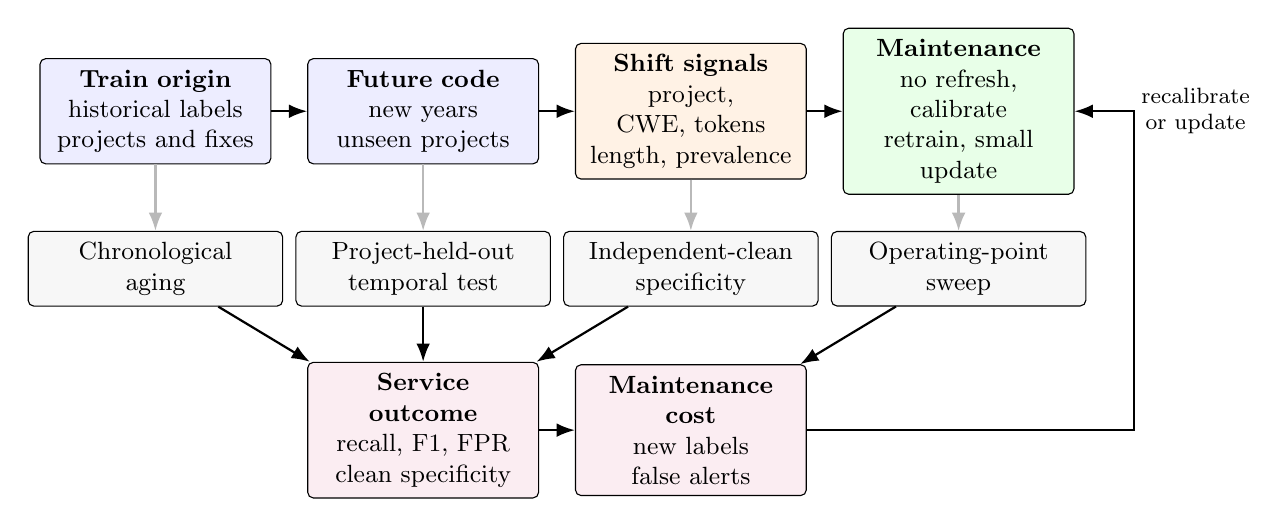
\begin{tikzpicture}[
    font=\small,
    flow/.style={draw, rounded corners=2pt, align=center, minimum height=0.9cm,
      text width=2.65cm, inner sep=4pt, fill=white},
    check/.style={draw, rounded corners=2pt, align=center, minimum height=0.78cm,
      text width=2.95cm, inner sep=4pt, fill=gray!6},
    outcome/.style={draw, rounded corners=2pt, align=center, minimum height=0.78cm,
      text width=2.65cm, inner sep=4pt, fill=white},
    arrow/.style={-Latex, thick},
    faint/.style={draw=gray!55, -Latex, thick}
  ]
    \node[flow, fill=blue!7] (origin) at (0,0)
      {\textbf{Train origin}\\ historical labels\\ projects and fixes};
    \node[flow, fill=blue!7] (future) at (3.4,0)
      {\textbf{Future code}\\ new years\\ unseen projects};
    \node[flow, fill=orange!10] (drift) at (6.8,0)
      {\textbf{Shift signals}\\ project, CWE, tokens\\ length, prevalence};
    \node[flow, fill=green!9] (policy) at (10.2,0)
      {\textbf{Maintenance}\\ no refresh, calibrate\\ retrain, small update};

    \node[check] (chrono) at (0,-2.0) {Chronological\\aging};
    \node[check] (holdout) at (3.4,-2.0) {Project-held-out\\temporal test};
    \node[check] (clean) at (6.8,-2.0) {Independent-clean\\specificity};
    \node[check] (threshold) at (10.2,-2.0) {Operating-point\\sweep};

    \node[outcome, fill=purple!7] (service) at (3.4,-4.05)
      {\textbf{Service outcome}\\ recall, F1, FPR\\ clean specificity};
    \node[outcome, fill=purple!7] (cost) at (6.8,-4.05)
      {\textbf{Maintenance cost}\\ new labels\\ false alerts};

    \draw[arrow] (origin) -- (future);
    \draw[arrow] (future) -- (drift);
    \draw[arrow] (drift) -- (policy);
    \draw[faint] (origin) -- (chrono);
    \draw[faint] (future) -- (holdout);
    \draw[faint] (drift) -- (clean);
    \draw[faint] (policy) -- (threshold);
    \draw[arrow] (chrono) -- (service);
    \draw[arrow] (holdout) -- (service);
    \draw[arrow] (clean) -- (service);
    \draw[arrow] (threshold) -- (cost);
    \draw[arrow] (service) -- (cost);
    \draw[arrow] (cost.east) -- ++(4.15,0) coordinate (loopright)
      |- node[pos=0.66,right,font=\footnotesize,align=center]
      {recalibrate\\or update}
      ([xshift=0.65cm]policy.east) -- (policy.east);
  \end{tikzpicture}
  \caption{Visual summary of MAINT-VD detector maintenance.}
  \label{fig:maintenance-loop}
\end{figure*}

\section{Experimental Design}

\subsection{Datasets}

Table~\ref{tab:datasets} summarizes the temporal exports. CVEfixes is the
primary source because the local mirror contains explicit temporal metadata.
The normalizer converts \texttt{vulnerable\_code} into positive records and
\texttt{fixed\_code} into negative records. This construction supports temporal
maintenance analysis of a pre/post-fix detector, but it should not be read as
arbitrary vulnerable-versus-clean classification.

DiverseVul is included as recovered-date sensitivity evidence. The available
local mirror does not expose explicit commit dates, so using it directly would
force a coarse CVE-year proxy and skip many raw rows. We therefore
join the mirror to the official DiverseVul metadata file, which contains
repository and commit URLs. The join matches 45,402 local rows. A broader HTTP
recovery pass over GitHub commit pages and known mirrors recovers commit dates
for 1,008 project/commit pairs, covering 37,767 rows before deduplication. After
truncation and exact-duplicate removal, the recovered-date subset contains
37,425 rows. Rows without recovered dates are excluded from recovered-date
temporal claims rather than mixed with proxy dates. The recovered-date filter
also narrows project diversity: the sensitivity subset contains 156 projects,
so DiverseVul is used as recovered-date sensitivity evidence rather than as a
claim of broad project coverage.

PrimeVul-paired is added as a third external sensitivity dataset after commit
date recovery. The public paired mirror includes commit identifiers and commit
URLs but no explicit timestamp column. We therefore fetch commit pages and
extract commit timestamps, recovering dates for 494 commit pages. This yields
1,393 timestamped rows before exact deduplication and 1,267 rows after
deduplication. The evidence is stronger than the earlier CVE-year proxy check
because the temporal split is commit-dated, but the task is still paired
pre/post-fix detection and is not treated as independent clean-code
classification.

\begin{table*}
\centering
\caption{Temporal exports after exact duplicate removal.}
\label{tab:datasets}
\resizebox{\textwidth}{!}{%
\begin{tabular}{lrrrrrr}
\toprule
Dataset & Years & Records & Removed duplicates & Vulnerable & Non-vulnerable & Projects \\
\midrule
CVEfixes & 1999--2024 & 19,791 & 2,269 & 8,976 & 10,815 & 3,836 \\
DiverseVul recovered dates & 2005--2022 & 37,425 & 342 & 2,378 & 35,047 & 156 \\
PrimeVul-paired recovered dates & 2009--2022 & 1,267 & 126 & 627 & 640 & 74 \\
\bottomrule
\end{tabular}
}
\end{table*}

\begin{table*}
\centering
\caption{DiverseVul recovered-date accounting.}
\label{tab:diversevul-accounting}
\small
\begin{tabular}{lrrl}
\toprule
Pipeline stage & Rows & Projects or pairs & Notes \\
\midrule
Local normalized DiverseVul mirror & 48,245 & 223 projects & Before date recovery \\
Matched to official metadata & 45,402 & 1,193 project/commit pairs & Repository and commit URLs available \\
Recovered commit dates & 37,767 & 1,008 project/commit pairs & 10,478 rows still lack recovered dates \\
After truncation and exact deduplication & 37,425 & 156 projects & 342 exact duplicates removed \\
Fixed-origin temporal span, 2009--2022 & 37,143 & 156 projects & Train/validation/test years used below \\
\bottomrule
\end{tabular}
\end{table*}

\subsection{Temporal Splits}

The corrected CVEfixes run trains on 2010--2016, validates on 2017, and tests
on 2018--2024. The recovered-date DiverseVul run trains on 2009--2015,
validates on 2016, and tests on 2017--2022. Both runs require minimum positive
and negative counts in the training, validation, and test windows.

For sensitivity, we rerun CVEfixes over four cutoffs:
2009--2015/2016/2017--2024, 2010--2016/2017/2018--2024,
2011--2017/2018/2019--2024, and 2012--2018/2019/2020--2024. This tests whether
the CVEfixes stability claim depends on a single temporal origin. The
rolling-origin drift analysis uses the same four CVEfixes origins and the
analogous recovered-date DiverseVul origins:
2009--2014/2015/2016--2022, 2009--2015/2016/2017--2022,
2009--2016/2017/2018--2022, and 2009--2017/2018/2019--2022, yielding 22
DiverseVul future-year pairs.

The temporal design has two variants. The ordinary temporal variant evaluates
all examples in the future year after exact duplicate removal. This measures
future-window behavior under the same broad project population. The
project-held-out temporal variant removes validation and test examples whose
project appeared in the relevant training window. For no-refresh and
calibration-only policies, the exclusion set is the original training-period
project set. For cumulative, sliding-window, and small-update policies, the
exclusion set is the full set of projects eligible for the policy's training
or update data; any sampling used to bound model-fitting cost does not weaken
the project-holdout definition.

\subsection{Detector Families}

The lightweight baselines are deterministic and inspectable:

\begin{itemize}
  \item \texttt{token\_tfidf\_logreg}: token TF-IDF features with logistic
  regression.
  \item \texttt{char4\_hash\_logreg}: hashed character 4-gram features with
  logistic regression.
  \item \texttt{code\_metrics\_logreg}: source-code metrics and security-token
  counts with logistic regression.
  \item \texttt{frozen\_hash\_embedding\_logreg}: deterministic frozen
  random-indexing features with a trained logistic head.
\end{itemize}

We designate \texttt{char4\_hash\_logreg} as the primary low-compute baseline
because it is language-agnostic and robust to tokenization differences. This is
a protocol choice recorded in the released analysis scripts, not an external
OSF-style preregistration. To address detector-family validity, we also
evaluate frozen CodeBERT embeddings with a logistic head, a pretrained
LineVul-style classifier calibrated on the validation year, and full-dataset
fine-tuning of CodeBERT and LineVul.

Exploratory bounded fine-tuning runs update all transformer layers but use only
400 balanced training rows, 300 validation rows, 150 test rows per future year,
one epoch, and maximum sequence length 128. They are retained in the artifact
as execution checks and are not used for comparative claims. The stricter
full-dataset neural setting uses all temporal training rows, filters validation
and future test to projects unseen during training years, and selects
thresholds on validation subject to a false-positive-rate ceiling of 0.20 when
feasible. We therefore interpret neural results through operating-point curves
rather than a single selected threshold.

\subsection{Maintenance Policies and Operating Points}

The maintenance-policy experiment treats a detector as a software artifact
that can be refreshed in different ways after deployment. The no-refresh policy
keeps the original model and threshold. Cumulative retraining uses all
available years up to two years before the target test year, then calibrates on
the immediately preceding year. Sliding-window retraining uses the three most
recent eligible years before calibration. Calibration-only keeps the original
model weights but reselects the decision threshold on recent validation data.
Small recent update appends a bounded number of recent positive and negative
examples to the original training set before refitting. We add a
vulnerability-specific policy, CWE-aware sliding retraining, that starts from
the three-year sliding window and oversamples weakness classes whose positive
share has increased in the most recent labeled calibration year. The policy is
not allowed to inspect the target test year; it uses the recent labeled year to
adapt the update batch toward shifted CWE prevalence.

Operating points are selected on validation data only. For classical aging and
maintenance summaries, the default threshold maximizes validation F1. For the
full-dataset neural project-held-out experiment, the threshold is selected
subject to a validation false-positive-rate ceiling of 0.20 when feasible; if
the ceiling is infeasible, the lowest-FPR candidate is reported. To avoid
hiding this design choice, neural results also include threshold sweeps with
precision, recall, F1, specificity, FPR, AUROC, and AUPRC\@. The article treats
recall gains without FPR context as incomplete maintenance evidence.
In the reported full-dataset neural runs, the FPR ceiling is feasible for all
four validation selections. The recovered-date DiverseVul neural rows have
validation FPR 0.000 because the selected threshold predicts no positives on
validation, not because the ceiling is infeasible. For this imbalanced
project-held-out setting, the fixed-FPR rule is therefore treated as
mis-specified: it can satisfy the service ceiling by suppressing nearly all
positive predictions. A proper neural rerun should compare this rule with
precision-floor, best-F1, and Youden-\(J\) threshold policies and report the
full validation precision-recall surface.

\subsection{Leakage and Validity Controls}

Exact canonical duplicate functions are removed before splitting. We also run a
near-duplicate control that preserves the training origin and removes
validation or test records whose SimHash is within Hamming distance 3 of an
earlier kept record and whose token-count ratio is between 0.75 and 1.33. The
recovered-date DiverseVul validity pass finds 10,623 near-duplicate candidate
pairs after exact deduplication, while grouped analysis reports no train-to-test
commit-group or pair-group overlap.

To test whether fixed-code negatives substitute for independently clean code,
we construct a repository-clean benchmark from local research software and
external C/C++ repositories outside the vulnerability-dataset construction
pipeline. The extractor keeps Python and C-like functions, removes exact
canonical overlap with CVEfixes, recovered-date DiverseVul, and PrimeVul-paired,
and caps per-project contribution. The resulting benchmark contains 2,500
functions from 39 project/source groups: 2,265 C/C++-family functions and 235
Python functions. These projects are not claimed to be formally defect-free; the
point is narrower and stronger than the earlier dataset-derived stress test:
the clean examples are not derived from vulnerability-fixing commits and do not
reuse the temporal vulnerability datasets' negative-example construction.

\subsection{Statistical Protocol}

The statistical protocol is descriptive because the number of annual future
windows is small. We therefore focus on effect sizes and uncertainty intervals
rather than binary significance claims. For fixed-origin aging, the primary
effect is the change between the first and last future windows and the mean
future score over all test years. For maintenance policies, the primary effect
is the paired difference from no refresh in each future year, reported with
mean recall, mean F1, mean FPR, and mean label cost per window.

Uncertainty intervals for policy summaries are non-parametric bootstrap
intervals over yearly windows using 1,000 resamples and the 2.5th and 97.5th
percentiles. Drift-performance links are evaluated with rolling-origin paired
replicates rather than only one fixed origin. We reuse the four CVEfixes cutoff
origins from the temporal sensitivity analysis and add the analogous four
recovered-date DiverseVul origins listed in Section~4.2. Each future test year
under each origin contributes one paired row containing drift signals and recall
drop from that origin's first future window, yielding 26 CVEfixes pairs and 22
DiverseVul pairs. Pearson correlations are checked with permutation tests that
shuffle the paired performance sequence while preserving the drift series. For
each dataset, the nine drift-signal tests are adjusted with the Holm procedure,
and correlation intervals are reported with Fisher's $z$-transform. The tests
are interpreted as associations, not causality. For neural
operating-point analysis, AUROC and AUPRC summarize ranking quality, while
threshold-specific precision, recall, F1, specificity, and FPR summarize
deployment behavior at candidate operating points.

To keep the claims falsifiable, we also state two operating-point decision
criteria. C1 asks whether small recent updates increase recall by at least 0.05
over no refresh on CVEfixes under unseen-project temporal testing while keeping
future FPR at or below 0.20. C2 asks whether any recovered-date DiverseVul
maintenance policy maintains recall at least 0.50 with future FPR at or below
0.30 across future windows. The current results do not pass C1 because the
CVEfixes recall gain is coupled to FPR 0.945, and they do not identify a
DiverseVul policy that satisfies the C2 service level. This framing turns the
maintenance thesis into explicit service-level tests rather than a general claim
that all update policies help.

\section{Results}

Table~\ref{tab:intro-findings} provides the summary anchor for the results.
The subsections below give the detailed evidence behind those findings:
fixed-origin temporal
behavior and cutoff sensitivity, project-held-out policy tradeoffs,
repository-clean specificity, neural operating-point diagnostics, rolling-origin
drift correlations, and ordinary-temporal maintenance summaries.

\subsection{RQ1: Fixed-Origin Temporal Behavior}

\rqsummary{CVEfixes shows stable pre/post-fix recall for the primary character
baseline, but the high temporal FPR and low repository-clean specificity limit
any operational interpretation. Recovered-date DiverseVul is more volatile,
showing that temporal behavior depends on dataset construction and operating
point.}

Table~\ref{tab:aging} reports fixed-origin aging summaries. CVEfixes does not
show catastrophic aging for the primary character baseline under the
corrected split: mean future recall is 0.882 [0.871, 0.893], but temporal FPR
is 0.821 and independent-clean specificity is 0.155 [0.142, 0.170].
These are pre/post-fix detection scores and are not interpreted as arbitrary
vulnerable-versus-clean deployment performance.
The recovered-date DiverseVul subset is more volatile: the same baseline has
mean future recall 0.455 [0.371, 0.556] with temporal FPR 0.252 and
independent-clean specificity 0.700 [0.682, 0.718]. This contrast is central to
the article's claim. Temporal behavior is dataset- and policy-dependent; the
maintenance problem is to measure that behavior and choose an operating policy,
not to assume universal monotonic decay.

\begin{table*}
\centering
\caption{Headline temporal and independent-clean endpoints.}
\label{tab:aging}
\small
\setlength{\tabcolsep}{4pt}
\begin{tabular}{llp{0.15\textwidth}rrp{0.15\textwidth}r}
\toprule
Dataset & Model & Mean recall [95\% CI] & Mean F1 & Temporal FPR &
Clean specificity [95\% CI] & Clean FPR \\
\midrule
CVEfixes & char4 hash LR & 0.882 [0.871, 0.893] & 0.619 & 0.821 & 0.155 [0.142, 0.170] & 0.845 \\
CVEfixes & code metrics LR & 0.904 [0.892, 0.917] & 0.633 & 0.804 & 0.075 [0.065, 0.086] & 0.925 \\
CVEfixes & frozen emb. LR & 0.820 [0.808, 0.831] & 0.628 & 0.669 & 0.275 [0.258, 0.293] & 0.725 \\
CVEfixes & token TF-IDF LR & 0.851 [0.833, 0.868] & 0.653 & 0.637 & 0.184 [0.170, 0.200] & 0.816 \\
\midrule
DiverseVul recovered & char4 hash LR & 0.455 [0.371, 0.556] & 0.180 & 0.252 & 0.700 [0.682, 0.718] & 0.300 \\
DiverseVul recovered & code metrics LR & 0.655 [0.607, 0.702] & 0.215 & 0.307 & 0.825 [0.810, 0.840] & 0.175 \\
DiverseVul recovered & frozen emb. LR & 0.345 [0.323, 0.368] & 0.180 & 0.170 & 0.812 [0.796, 0.826] & 0.188 \\
DiverseVul recovered & token TF-IDF LR & 0.633 [0.599, 0.666] & 0.172 & 0.396 & 0.579 [0.560, 0.598] & 0.421 \\
\bottomrule
\end{tabular}
\end{table*}

Table~\ref{tab:cutoff-sensitivity} reports the CVEfixes cutoff sensitivity for
the primary character baseline. The ordinary-temporal stability claim is not an
artifact of a single origin: mean recall ranges from 0.884 to 0.978 across four
train/validation/test origins. The sign of first-to-last recall change varies,
which supports the article's narrower claim that temporal behavior is origin- and
policy-dependent rather than monotonically aging. In Table~\ref{tab:cutoff-sensitivity},
decay is first-test recall minus last-test recall, so negative values indicate
higher recall in the last test window.

\begin{table*}
\centering
\caption{CVEfixes cutoff sensitivity for the primary character baseline.}
\label{tab:cutoff-sensitivity}
\small
\setlength{\tabcolsep}{4pt}
\begin{tabular}{lrrrrr}
\toprule
Cutoff & First recall & Last recall & Decay & Worst recall & Mean recall \\
\midrule
2009--2015/2016/2017--2024 & 0.892 & 0.877 & 0.014 & 0.872 & 0.884 \\
2010--2016/2017/2018--2024 & 0.866 & 0.902 & -0.035 & 0.866 & 0.884 \\
2011--2017/2018/2019--2024 & 0.951 & 0.977 & -0.027 & 0.951 & 0.965 \\
2012--2018/2019/2020--2024 & 0.976 & 0.985 & -0.009 & 0.971 & 0.978 \\
\bottomrule
\end{tabular}
\end{table*}

Table~\ref{tab:primevul} adds PrimeVul-paired as a third external sensitivity
dataset with recovered commit dates. The commit-date subset is much smaller
than the full paired mirror because only 494 commit pages were recovered, but
its temporal split no longer depends on CVE-year proxy dates. The task remains
paired pre/post-fix detection rather than arbitrary vulnerable-versus-clean
detection. We therefore interpret the result as external temporal sensitivity
evidence: classical detectors again show that recall on paired
vulnerable/fixed examples must be interpreted jointly with alert cost and
independent-clean specificity.

\begin{table*}
\centering
\caption{PrimeVul-paired recovered-date fixed-origin sensitivity.}
\label{tab:primevul}
\small
\setlength{\tabcolsep}{4pt}
\begin{tabular}{lp{0.13\textwidth}p{0.13\textwidth}p{0.15\textwidth}p{0.15\textwidth}p{0.15\textwidth}}
\toprule
Model & First recall & Last recall & Mean recall [95\% CI] & Mean F1 [95\% CI] & Mean FPR [95\% CI] \\
\midrule
char4 hash LR & 0.726 & 1.000 & 0.789 [0.675, 0.910] & 0.625 [0.585, 0.666] & 0.776 [0.679, 0.891] \\
code metrics LR & 1.000 & 1.000 & 1.000 [1.000, 1.000] & 0.685 [0.660, 0.716] & 0.998 [0.995, 1.000] \\
frozen emb. LR & 0.938 & 1.000 & 0.939 [0.905, 0.973] & 0.671 [0.653, 0.688] & 0.932 [0.883, 0.972] \\
token TF-IDF LR & 0.779 & 0.900 & 0.810 [0.758, 0.866] & 0.639 [0.617, 0.666] & 0.779 [0.662, 0.906] \\
\bottomrule
\end{tabular}
\end{table*}

Table~\ref{tab:cross-dataset} adds a compact cross-dataset probe for the
primary character model. Each row trains and calibrates on one dataset's
historical window, then tests on future windows from another recovered-date
dataset. The results should be read as a stress test of dataset bias, not as a
new primary benchmark. Cross-dataset recall is possible, but FPR and F1 vary
substantially; this reinforces the article's claim that dataset construction and
operating point are part of detector maintenance.

\begin{table*}
\centering
\caption{Cross-dataset temporal probe for the primary character model.}
\label{tab:cross-dataset}
\small
\setlength{\tabcolsep}{5pt}
\begin{tabular}{llrrrr}
\toprule
Train/calibration source & Future test source & Windows & Mean recall & Mean F1 & Mean FPR \\
\midrule
CVEfixes & DiverseVul recovered & 6 & 0.883 & 0.130 & 0.861 \\
CVEfixes & PrimeVul recovered & 5 & 0.912 & 0.653 & 0.892 \\
PrimeVul recovered & DiverseVul recovered & 6 & 0.821 & 0.135 & 0.769 \\
DiverseVul recovered & PrimeVul recovered & 5 & 0.322 & 0.394 & 0.300 \\
\bottomrule
\end{tabular}
\end{table*}

Table~\ref{tab:project-maintenance} repeats the five standard classical
policies and the CWE-aware sliding policy under
unseen-project temporal testing. This design is the strongest classical
policy-validity check because it asks whether maintenance helps on projects not
seen during training. On CVEfixes, refresh and calibration policies increase
recall over no refresh, but mean FPR remains between 0.932 and 0.945. The recall
gain therefore buys more detected positives at substantial alert cost. The
CWE-aware policy slightly lowers CVEfixes FPR relative to the other refresh
policies, but it does not solve the alert-cost problem. On recovered-date
DiverseVul, refresh policies reduce FPR while also reducing recall. The C2
criterion is therefore a negative result: no tested policy reaches recall
\(\geq 0.50\) while keeping FPR \(\leq 0.30\). Across both datasets,
maintenance policy, label cost, and operating point must be interpreted
together.

\begin{table*}
\centering
\caption{Classical maintenance policies under unseen-project temporal testing.}
\label{tab:project-maintenance}
\resizebox{\textwidth}{!}{%
\begin{tabular}{llrrrrr}
\toprule
Dataset & Policy & Mean recall & Recall CI & Mean F1 & Mean FPR & Labels/window \\
\midrule
CVEfixes & No refresh & 0.935 & [0.925, 0.944] & 0.629 & 0.890 & 0.0 \\
CVEfixes & Cumulative retrain & 0.970 & [0.953, 0.985] & 0.638 & 0.938 & 975.9 \\
CVEfixes & Sliding 3-year retrain & 0.971 & [0.957, 0.983] & 0.638 & 0.944 & 1021.0 \\
CVEfixes & Calibration only & 0.972 & [0.951, 0.988] & 0.633 & 0.944 & 1529.3 \\
CVEfixes & Small recent update & 0.972 & [0.948, 0.989] & 0.637 & 0.945 & 40.0 \\
CVEfixes & CWE-aware sliding & 0.966 & [0.953, 0.978] & 0.638 & 0.932 & 1021.0 \\
\midrule
DiverseVul recovered & No refresh & 0.943 & [0.893, 0.976] & 0.149 & 0.860 & 0.0 \\
DiverseVul recovered & Cumulative retrain & 0.424 & [0.196, 0.675] & 0.158 & 0.291 & 1546.8 \\
DiverseVul recovered & Sliding 3-year retrain & 0.379 & [0.173, 0.632] & 0.162 & 0.243 & 1573.8 \\
DiverseVul recovered & Calibration only & 0.435 & [0.219, 0.700] & 0.152 & 0.315 & 2397.7 \\
DiverseVul recovered & Small recent update & 0.347 & [0.164, 0.522] & 0.174 & 0.195 & 40.0 \\
DiverseVul recovered & CWE-aware sliding & 0.430 & [0.276, 0.655] & 0.175 & 0.290 & 1573.8 \\
\bottomrule
\end{tabular}
}
\end{table*}

Table~\ref{tab:small-budget} isolates the small-update label budget because
reviewers reasonably asked whether the pre-specified 40-label setting is an
arbitrary sweet spot. It is deliberately modest: each future window receives at
most 20 newly labeled positives and 20 newly labeled negatives, approximating a
lightweight periodic triage batch rather than full retraining. The sensitivity
run shows that budgets from 10 to 200 labels/window barely change the service
profile. The method preserves high recall, but high FPR remains; in this
setting the limiting factor is the operating point and project shift, not the
exact small-update budget.

\begin{table*}
\centering
\caption{CVEfixes project-held-out small-update budget sensitivity.}
\label{tab:small-budget}
\small
\setlength{\tabcolsep}{4pt}
\begin{tabular}{rrrrl}
\toprule
Labels/window & Recall & Mean F1 & Mean FPR & Interpretation \\
\midrule
10 & 0.973 [0.952, 0.988] & 0.637 & 0.947 & High recall, high alert cost \\
40 & 0.972 [0.948, 0.989] & 0.637 & 0.945 & Pre-specified budget \\
100 & 0.973 [0.949, 0.991] & 0.637 & 0.946 & No material gain \\
200 & 0.966 [0.947, 0.986] & 0.636 & 0.941 & Slightly lower FPR \\
\bottomrule
\end{tabular}
\end{table*}

Table~\ref{tab:primevul-neural} and Figure~\ref{fig:primevul-training}
report the tuned neural diagnostic rerun requested by the review analysis. The
rerun uses full-parameter fine-tuning, the recovered-date PrimeVul subset, all
eligible training, validation, and test rows under future-project holdout, maximum
sequence length 256, class-balanced loss, five requested epochs, early stopping
by validation AUPRC, and retained validation-threshold curves. It is still a
diagnostic rather than a definitive architecture comparison, but it is no
longer a tiny capped run: both models train on all 499 eligible historical rows
and are tested on all 329 eligible future unseen-project rows. The curves show
limited learnability rather than a silent pipeline failure. CodeBERT reaches
moderate validation AUPRC but the selected FPR-controlled threshold predicts
almost all future examples negative; LineVul reaches a nonzero validation
operating point but pays higher future FPR.

\begin{table*}
\centering
\caption{PrimeVul-paired recovered-date neural diagnostic rerun.}
\label{tab:primevul-neural}
\small
\setlength{\tabcolsep}{4pt}
\begin{tabular}{p{0.16\textwidth}p{0.19\textwidth}p{0.20\textwidth}p{0.33\textwidth}}
\toprule
Model & Sample and epoch & Validation operating point & Future test behavior \\
\midrule
CodeBERT full FT & Train/val/test 499/57/329; best epoch 1 &
AUPRC 0.573; selected recall/FPR 0.000/0.000 &
Recall 0.015 [0.000, 0.037]; F1 0.027 [0.000, 0.066]; FPR 0.014 [0.000, 0.034] \\
LineVul full FT & Train/val/test 499/57/329; best epoch 3 &
AUPRC 0.554; selected recall/FPR 0.250/0.172 &
Recall 0.234 [0.084, 0.376]; F1 0.280 [0.134, 0.416]; FPR 0.227 [0.085, 0.376] \\
\bottomrule
\end{tabular}
\end{table*}

\begin{figure}
  \centering
  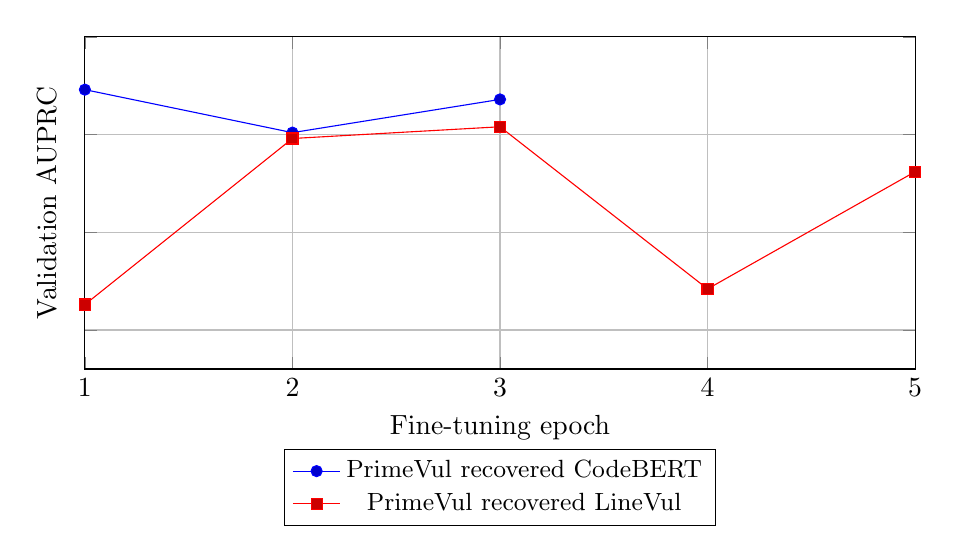
\begin{tikzpicture}
    \begin{axis}[
      width=\columnwidth,
      height=5.8cm,
      xmin=1,
      xmax=5,
      ymin=0.43,
      ymax=0.60,
      xlabel={Fine-tuning epoch},
      ylabel={Validation AUPRC},
      yticklabel=\empty,
      xtick={1,2,3,4,5},
      legend style={at={(0.5,-0.24)},anchor=north,font=\small},
      legend columns=1,
      grid=major
    ]
      \addplot+[blue,mark=*] coordinates {
        (1,0.573) (2,0.551) (3,0.568)
      };
      \addlegendentry{PrimeVul recovered CodeBERT}
      \addplot+[red,mark=square*] coordinates {
        (1,0.463) (2,0.548) (3,0.554) (4,0.471) (5,0.531)
      };
      \addlegendentry{PrimeVul recovered LineVul}
    \end{axis}
  \end{tikzpicture}
  \caption{PrimeVul-paired neural validation AUPRC by epoch.}
  \label{fig:primevul-training}
\end{figure}

\begin{figure}
  \centering
  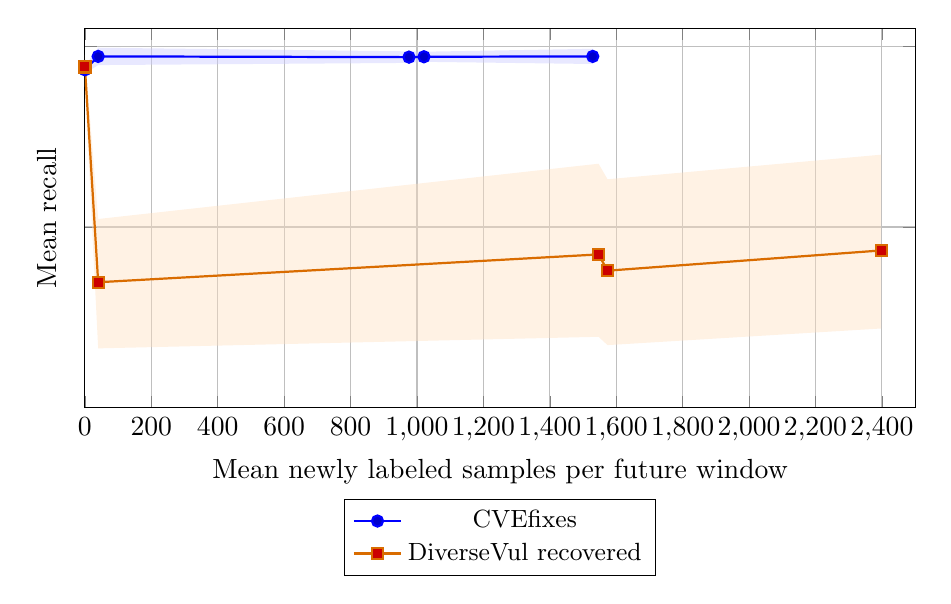
\begin{tikzpicture}
    \begin{axis}[
      width=\columnwidth,
      height=6.4cm,
      xmin=0,
      xmax=2500,
      ymin=0,
      ymax=1.05,
      xlabel={Mean newly labeled samples per future window},
      ylabel={Mean recall},
      yticklabel=\empty,
      legend style={at={(0.5,-0.24)},anchor=north,font=\small},
      legend columns=1,
      grid=major
    ]
      \addplot[name path=cvepolicycostupper,draw=none,forget plot] coordinates {
        (0,0.945) (40.0,0.996) (975.9,0.986) (1021.0,0.985) (1529.3,0.993)
      };
      \addplot[name path=cvepolicycostlower,draw=none,forget plot] coordinates {
        (0,0.925) (40.0,0.948) (975.9,0.954) (1021.0,0.957) (1529.3,0.951)
      };
      \addplot[blue!20,opacity=0.45,forget plot] fill between[of=cvepolicycostupper and cvepolicycostlower];
      \addplot+[blue,thick,mark=*] coordinates {
        (0,0.935) (40.0,0.972) (975.9,0.970) (1021.0,0.971) (1529.3,0.972)
      };
      \addlegendentry{CVEfixes}
      \addplot[name path=dvpolicycostupper,draw=none,forget plot] coordinates {
        (0,0.976) (40.0,0.522) (1546.8,0.675) (1573.8,0.632) (2397.7,0.700)
      };
      \addplot[name path=dvpolicycostlower,draw=none,forget plot] coordinates {
        (0,0.893) (40.0,0.164) (1546.8,0.196) (1573.8,0.173) (2397.7,0.219)
      };
      \addplot[orange!25,opacity=0.42,forget plot] fill between[of=dvpolicycostupper and dvpolicycostlower];
      \addplot+[orange!85!black,thick,mark=square*] coordinates {
        (0,0.943) (40.0,0.347) (1546.8,0.424) (1573.8,0.379) (2397.7,0.435)
      };
      \addlegendentry{DiverseVul recovered}
    \end{axis}
  \end{tikzpicture}
  \caption{Policy-vs-label-cost view under unseen-project temporal testing.}
  \label{fig:policy-cost}
\end{figure}

\begin{figure}
  \centering
  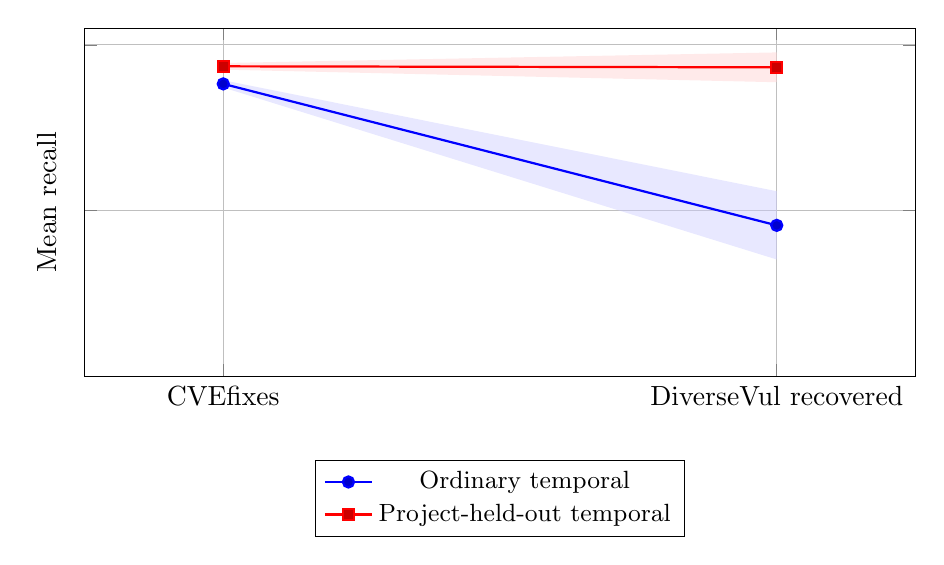
\begin{tikzpicture}
    \begin{axis}[
      width=\columnwidth,
      height=6cm,
      xmin=0.75,
      xmax=2.25,
      ymin=0,
      ymax=1.05,
      ylabel={Mean recall},
      yticklabel=\empty,
      xtick={1,2},
      xticklabels={CVEfixes,DiverseVul recovered},
      legend style={at={(0.5,-0.24)},anchor=north,font=\small},
      legend columns=1,
      grid=major
    ]
      \addplot[name path=ordinaryupper,draw=none,forget plot] coordinates {
        (1,0.893) (2,0.558)
      };
      \addplot[name path=ordinarylower,draw=none,forget plot] coordinates {
        (1,0.871) (2,0.352)
      };
      \addplot[blue!20,opacity=0.45,forget plot] fill between[of=ordinaryupper and ordinarylower];
      \addplot+[blue,thick,mark=*] coordinates {
        (1,0.882) (2,0.455)
      };
      \addlegendentry{Ordinary temporal}
      \addplot[name path=phoupper,draw=none,forget plot] coordinates {
        (1,0.945) (2,0.977)
      };
      \addplot[name path=pholower,draw=none,forget plot] coordinates {
        (1,0.925) (2,0.887)
      };
      \addplot[red!18,opacity=0.45,forget plot] fill between[of=phoupper and pholower];
      \addplot+[red,thick,mark=square*] coordinates {
        (1,0.935) (2,0.932)
      };
      \addlegendentry{Project-held-out temporal}
    \end{axis}
  \end{tikzpicture}
  \caption{Ordinary temporal versus project-held-out no-refresh evaluation.}
  \label{fig:ordinary-project}
\end{figure}

\begin{figure}
  \centering
  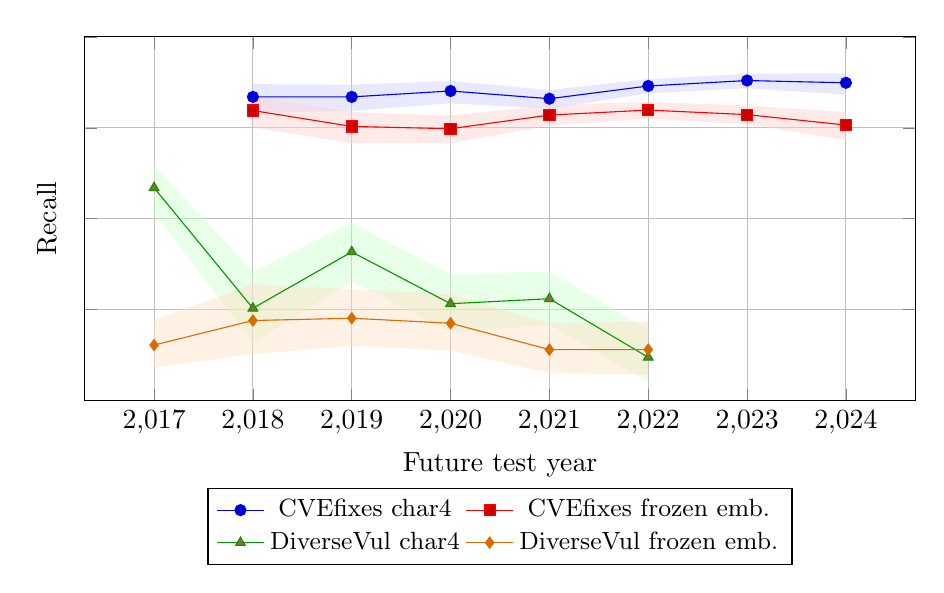
\begin{tikzpicture}
    \begin{axis}[
      width=\columnwidth,
      height=6.2cm,
      xlabel={Future test year},
      ylabel={Recall},
      yticklabel=\empty,
      ymin=0.20,
      ymax=1.00,
      xtick={2017,2018,2019,2020,2021,2022,2023,2024},
      legend style={at={(0.5,-0.24)},anchor=north,font=\small},
      legend columns=2,
      grid=both
    ]
      \addplot[name path=cvecharupper,draw=none,forget plot] coordinates {
        (2018,0.896) (2019,0.895) (2020,0.903) (2021,0.883)
        (2022,0.907) (2023,0.919) (2024,0.920)
      };
      \addplot[name path=cvecharlower,draw=none,forget plot] coordinates {
        (2018,0.834) (2019,0.837) (2020,0.854) (2021,0.842)
        (2022,0.876) (2023,0.887) (2024,0.873)
      };
      \addplot[blue!20,opacity=0.45,forget plot] fill between[of=cvecharupper and cvecharlower];
      \addplot[name path=cveembupper,draw=none,forget plot] coordinates {
        (2018,0.868) (2019,0.835) (2020,0.827) (2021,0.850)
        (2022,0.857) (2023,0.849) (2024,0.835)
      };
      \addplot[name path=cveemblower,draw=none,forget plot] coordinates {
        (2018,0.801) (2019,0.766) (2020,0.766) (2021,0.805)
        (2022,0.820) (2023,0.808) (2024,0.773)
      };
      \addplot[red!18,opacity=0.45,forget plot] fill between[of=cveembupper and cveemblower];
      \addplot[name path=dvcharupper,draw=none,forget plot] coordinates {
        (2017,0.718) (2018,0.483) (2019,0.591) (2020,0.478)
        (2021,0.484) (2022,0.356)
      };
      \addplot[name path=dvcharlower,draw=none,forget plot] coordinates {
        (2017,0.613) (2018,0.327) (2019,0.462) (2020,0.351)
        (2021,0.366) (2022,0.241)
      };
      \addplot[green!20,opacity=0.45,forget plot] fill between[of=dvcharupper and dvcharlower];
      \addplot[name path=dvembupper,draw=none,forget plot] coordinates {
        (2017,0.377) (2018,0.456) (2019,0.445) (2020,0.434)
        (2021,0.370) (2022,0.374)
      };
      \addplot[name path=dvemblower,draw=none,forget plot] coordinates {
        (2017,0.273) (2018,0.302) (2019,0.320) (2020,0.310)
        (2021,0.260) (2022,0.257)
      };
      \addplot[orange!24,opacity=0.45,forget plot] fill between[of=dvembupper and dvemblower];
      \addplot+[blue,mark=*] coordinates {
        (2018,0.868) (2019,0.868) (2020,0.881) (2021,0.864)
        (2022,0.892) (2023,0.904) (2024,0.899)
      };
      \addlegendentry{CVEfixes char4}
      \addplot+[red,mark=square*] coordinates {
        (2018,0.838) (2019,0.803) (2020,0.798) (2021,0.828)
        (2022,0.839) (2023,0.829) (2024,0.806)
      };
      \addlegendentry{CVEfixes frozen emb.}
      \addplot+[green!60!black,mark=triangle*] coordinates {
        (2017,0.668) (2018,0.403) (2019,0.527) (2020,0.413)
        (2021,0.424) (2022,0.295)
      };
      \addlegendentry{DiverseVul char4}
      \addplot+[orange!85!black,mark=diamond*] coordinates {
        (2017,0.322) (2018,0.376) (2019,0.381) (2020,0.370)
        (2021,0.312) (2022,0.312)
      };
      \addlegendentry{DiverseVul frozen emb.}
    \end{axis}
  \end{tikzpicture}
  \caption{Fixed-origin future recall curves with uncertainty bands.}
  \label{fig:aging}
\end{figure}

\subsection{Near-Duplicate-Controlled and Neural Reruns}

Table~\ref{tab:controlled-neural} reports the near-duplicate-controlled rerun
and lightweight neural-transfer sensitivities. The control does not reverse the
main interpretation: CVEfixes remains largely stable for the primary character
model, while DiverseVul continues to show substantial future recall decay.
Frozen CodeBERT embeddings are competitive on CVEfixes; the calibration-only
LineVul transfer baseline is weak. Bounded full fine-tuning is excluded from
the main comparison because the sampled one-epoch, length-128 setting is too
small to support a meaningful architecture claim.

\begin{table*}
\centering
\caption{Near-duplicate-controlled temporal sensitivity and lightweight
neural-transfer baselines.}
\label{tab:controlled-neural}
\resizebox{\textwidth}{!}{%
\begin{tabular}{llrrrr}
\toprule
Dataset & Model & First recall & Last recall & Mean recall & Mean F1 \\
\midrule
CVEfixes controlled & char4 hash LR & 0.868 & 0.899 & 0.882 & 0.619 \\
CVEfixes controlled & CodeBERT frozen emb. LR & 0.827 & 0.853 & 0.810 & 0.643 \\
CVEfixes controlled & LineVul calibrated & 0.147 & 0.240 & 0.166 & 0.229 \\
\midrule
DiverseVul recovered & char4 hash LR & 0.668 & 0.295 & 0.455 & 0.180 \\
\bottomrule
\end{tabular}
}
\end{table*}

Table~\ref{tab:full-project-holdout} reports the stricter neural experiment.
Unlike the bounded run, this design uses all training records, evaluates only
future projects absent from the training period, and caps validation FPR at
0.20 when selecting thresholds. On CVEfixes, CodeBERT retains moderate recall
and F1, while LineVul is more conservative. On recovered-date DiverseVul, the
same FPR-controlled thresholding rule drives both neural models to very low
recall. We therefore do not interpret the DiverseVul neural rows as evidence
that one architecture is better than another, nor as evidence that the
representation fails to rank examples. They are a diagnostic result: the
validation-FPR rule is mis-specified for this highly imbalanced
project-held-out regime because it can meet the FPR ceiling by selecting a
near-all-negative threshold.

\begin{table*}
\centering
\caption{Full-dataset neural fine-tuning under unseen-project temporal testing.}
\label{tab:full-project-holdout}
\scriptsize
\setlength{\tabcolsep}{3pt}
\begin{tabular}{llrrrrrrr}
\toprule
Dataset & Model & Train & Valid. & Test & Valid. recall & Valid. FPR & Mean recall & Mean F1 \\
\midrule
CVEfixes & CodeBERT full FT & 3,980 & 579 & 11,369 & 0.615 & 0.190 & 0.563 & 0.612 \\
CVEfixes & LineVul full FT & 3,980 & 579 & 11,369 & 0.452 & 0.183 & 0.414 & 0.503 \\
DiverseVul recovered & CodeBERT full FT & 11,208 & 874 & 15,724 & 0.000 & 0.000 & 0.000 & 0.000 \\
DiverseVul recovered & LineVul full FT & 11,208 & 874 & 15,724 & 0.000 & 0.000 & 0.006 & 0.011 \\
\bottomrule
\end{tabular}
\end{table*}

Table~\ref{tab:neural-operating} is treated as a primary result rather than an
appendix-style diagnostic: neural detector claims in this article are interpreted
through operating-point rules, not through a single selected threshold.
It expands the same neural runs across operating points, including best-F1,
FPR-controlled, precision-floor, and Youden-\(J\) policies computed from the
saved score distributions. On CVEfixes, CodeBERT has
higher AUROC and AUPRC than LineVul, but both models trade recall against
false-positive rate sharply as the threshold changes. At the best-F1 threshold,
CodeBERT reaches recall 0.816 at FPR 0.456 and F1 0.695; under the FPR20
operating point, recall falls to 0.481 at FPR 0.185 and F1 to 0.567. The
precision-floor policy recovers high recall on CVEfixes only by accepting high
FPR (0.812 for CodeBERT and 0.821 for LineVul). Recovered-date DiverseVul is
weaker under every threshold rule: CodeBERT's best-F1 and Youden-\(J\) points
both reach only recall 0.109 at FPR 0.028 and F1 0.145, while the
precision-floor rule is infeasible and falls back to precision 0.263 with
recall 0.020 at FPR 0.004. Thus the earlier zero-recall point was a threshold
artifact, but the rerun still shows no useful neural operating point on the
recovered-date project-held-out split.
In Table~\ref{tab:neural-operating}, FPR20 denotes validation-threshold
selection with FPR at most 0.20, and PF50 denotes the best available
precision-floor point at precision at least 0.50, falling back to the
highest-precision non-empty point when the floor is infeasible.

\begin{table*}
\centering
\caption{Operating-point summary for full-dataset project-held-out neural runs.}
\label{tab:neural-operating}
\scriptsize
\setlength{\tabcolsep}{3pt}
\resizebox{\textwidth}{!}{%
\begin{tabular}{llrrrrrr}
\toprule
Dataset & Model & AUROC & AUPRC & Best-F1 R/FPR & FPR20 R/FPR &
PF50 P/R/FPR & Youden R/FPR \\
\midrule
CVEfixes & CodeBERT full FT & 0.737 & 0.682 & 0.816/0.456 & 0.481/0.185 & 0.504/0.960/0.812 & 0.727/0.359 \\
CVEfixes & LineVul full FT & 0.688 & 0.618 & 0.862/0.632 & 0.426/0.197 & 0.501/0.956/0.821 & 0.640/0.356 \\
DiverseVul recovered & CodeBERT full FT & 0.724 & 0.149 & 0.109/0.028 & 0.109/0.028 & 0.263/0.020/0.004 & 0.109/0.028 \\
DiverseVul recovered & LineVul full FT & 0.696 & 0.124 & 1.000/1.000 & 0.021/0.008 & 0.222/0.004/0.001 & 0.021/0.008 \\
\bottomrule
\end{tabular}
}
\end{table*}

\begin{figure}
  \centering
  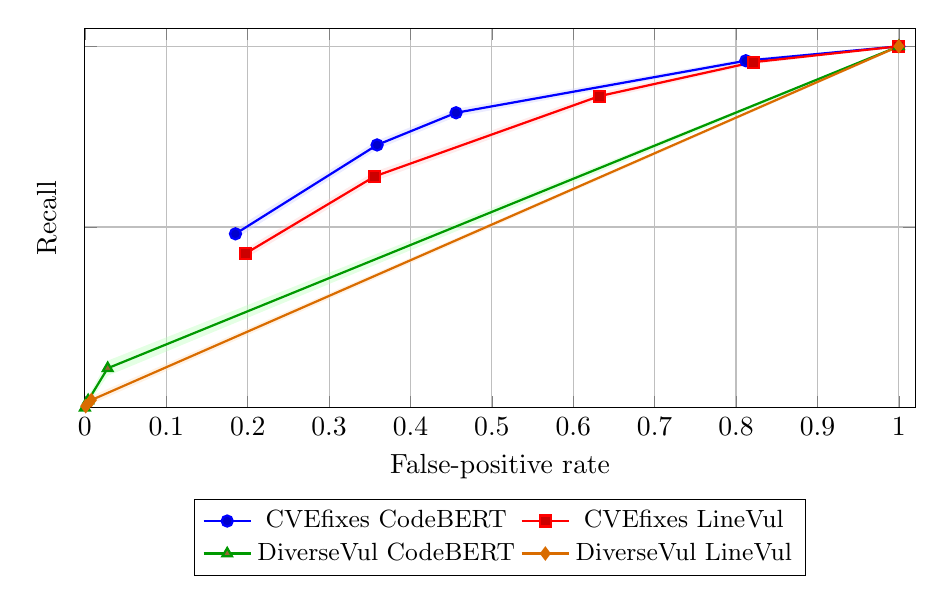
\begin{tikzpicture}
    \begin{axis}[
      width=\columnwidth,
      height=6.4cm,
      xmin=0,
      xmax=1.02,
      ymin=0,
      ymax=1.05,
      xlabel={False-positive rate},
      ylabel={Recall},
      yticklabel=\empty,
      legend style={at={(0.5,-0.24)},anchor=north,font=\small},
      legend columns=2,
      grid=major
    ]
      \addplot[name path=cvebertupper,draw=none,forget plot] coordinates {
        (0.185,0.495) (0.359,0.739) (0.456,0.827) (0.812,0.966) (1.000,1.000)
      };
      \addplot[name path=cvebertlower,draw=none,forget plot] coordinates {
        (0.185,0.467) (0.359,0.715) (0.456,0.805) (0.812,0.954) (1.000,0.999)
      };
      \addplot[blue!18,opacity=0.42,forget plot] fill between[of=cvebertupper and cvebertlower];
      \addplot+[blue,thick,mark=*] coordinates {
        (0.185,0.481) (0.359,0.727) (0.456,0.816) (0.812,0.960) (1.000,1.000)
      };
      \addlegendentry{CVEfixes CodeBERT}
      \addplot[name path=cvelineupper,draw=none,forget plot] coordinates {
        (0.197,0.439) (0.356,0.653) (0.632,0.872) (0.821,0.962) (1.000,1.000)
      };
      \addplot[name path=cvelinelower,draw=none,forget plot] coordinates {
        (0.197,0.413) (0.356,0.627) (0.632,0.852) (0.821,0.950) (1.000,0.999)
      };
      \addplot[red!18,opacity=0.42,forget plot] fill between[of=cvelineupper and cvelinelower];
      \addplot+[red,thick,mark=square*] coordinates {
        (0.197,0.426) (0.356,0.640) (0.632,0.862) (0.821,0.956) (1.000,1.000)
      };
      \addlegendentry{CVEfixes LineVul}
      \addplot[name path=dvbertupper,draw=none,forget plot] coordinates {
        (0.000,0.004) (0.004,0.030) (0.028,0.130) (1.000,1.000)
      };
      \addplot[name path=dvbertlower,draw=none,forget plot] coordinates {
        (0.000,0.000) (0.004,0.010) (0.028,0.088) (1.000,0.996)
      };
      \addplot[green!25,opacity=0.42,forget plot] fill between[of=dvbertupper and dvbertlower];
      \addplot+[green!60!black,thick,mark=triangle*] coordinates {
        (0.000,0.000) (0.004,0.020) (0.028,0.109) (1.000,1.000)
      };
      \addlegendentry{DiverseVul CodeBERT}
      \addplot[name path=dvlineupper,draw=none,forget plot] coordinates {
        (0.001,0.010) (0.008,0.032) (1.000,1.000)
      };
      \addplot[name path=dvlinelower,draw=none,forget plot] coordinates {
        (0.001,0.000) (0.008,0.010) (1.000,0.996)
      };
      \addplot[orange!25,opacity=0.42,forget plot] fill between[of=dvlineupper and dvlinelower];
      \addplot+[orange!85!black,thick,mark=diamond*] coordinates {
        (0.001,0.004) (0.008,0.021) (1.000,1.000)
      };
      \addlegendentry{DiverseVul LineVul}
    \end{axis}
  \end{tikzpicture}
  \caption{Threshold/FPR tradeoff for project-held-out neural runs.}
  \label{fig:operating}
\end{figure}

\subsection{Independent Clean and Grouped Validity}

Table~\ref{tab:clean} summarizes grouped and independent-clean checks. The
near-duplicate-controlled runs have no train-to-future commit-group or paired
vulnerable/fixed-group overlap. Project overlap is low in future CVEfixes test
windows and moderate in recovered-date DiverseVul. The repository-clean
benchmark gives the strongest warning: the CVEfixes-trained character model has
specificity 0.155 on clean functions harvested from projects outside the
vulnerability-dataset construction pipeline. This confirms that fixed-code
negatives do not substitute for independently sampled clean functions.

\begin{table*}
\centering
\caption{Grouped validity and independent-clean specificity.}
\label{tab:clean}
\small
\setlength{\tabcolsep}{4pt}
\begin{tabular}{lrrrrr}
\toprule
Dataset & Test project overlap & Commit overlap & Pair overlap &
Unseen-project recall & Clean specificity \\
\midrule
CVEfixes controlled & 0.046 & 0.000 & 0.000 & 0.891 & 0.155 \\
DiverseVul recovered & 0.102 & 0.000 & 0.000 & 0.494 & 0.700 \\
\bottomrule
\end{tabular}
\end{table*}

Table~\ref{tab:clean-source} reports the repository-clean benchmark by detector
family with Wilson confidence intervals. The CVEfixes-trained detectors have
poor specificity across all four feature families, ranging from 0.075 to 0.275.
Recovered-date DiverseVul is less uniformly poor: code metrics, frozen
embeddings, and character features have specificity between 0.700 and 0.825,
while token TF-IDF still flags many repository-clean functions. The key validity
point remains: a model can look
strong on pre/post-fix temporal recall while flagging many clean-only functions.

\begin{table*}
\centering
\caption{Repository-clean specificity by detector family.}
\label{tab:clean-source}
\small
\setlength{\tabcolsep}{4pt}
\begin{tabular}{llrrrr}
\toprule
Training source & Model & Rows & Specificity & 95\% CI & FPR \\
\midrule
CVEfixes & char4 hash LR & 2500 & 0.155 & [0.142, 0.170] & 0.845 \\
CVEfixes & code metrics LR & 2500 & 0.075 & [0.065, 0.086] & 0.925 \\
CVEfixes & frozen emb. LR & 2500 & 0.275 & [0.258, 0.293] & 0.725 \\
CVEfixes & token TF-IDF LR & 2500 & 0.184 & [0.170, 0.200] & 0.816 \\
\midrule
DiverseVul recovered & char4 hash LR & 2500 & 0.700 & [0.682, 0.718] & 0.300 \\
DiverseVul recovered & code metrics LR & 2500 & 0.825 & [0.810, 0.840] & 0.175 \\
DiverseVul recovered & frozen emb. LR & 2500 & 0.812 & [0.796, 0.826] & 0.188 \\
DiverseVul recovered & token TF-IDF LR & 2500 & 0.579 & [0.560, 0.598] & 0.421 \\
\bottomrule
\end{tabular}
\end{table*}

\begin{figure}
  \centering
  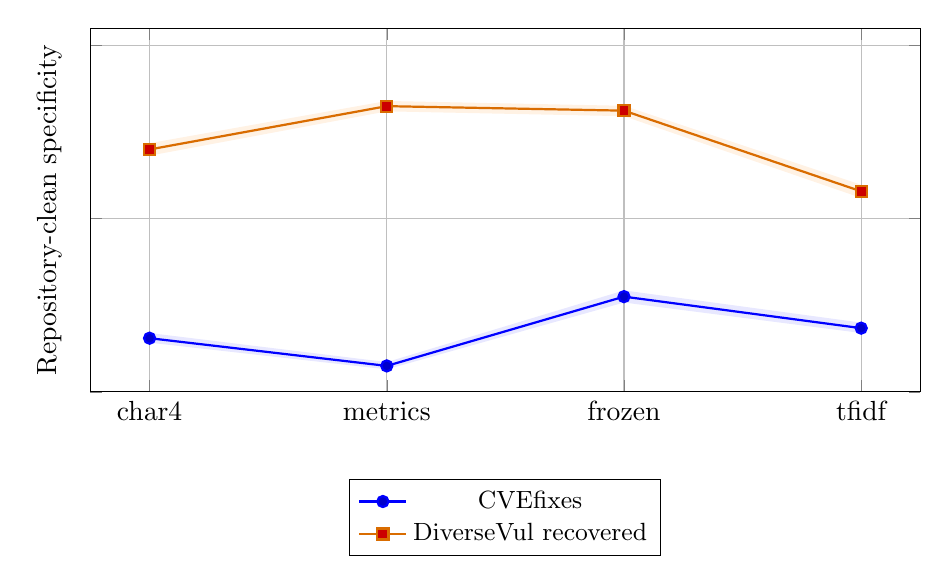
\begin{tikzpicture}
    \begin{axis}[
      width=\columnwidth,
      height=6.2cm,
      xmin=0.75,
      xmax=4.25,
      ymin=0,
      ymax=1.05,
      ylabel={Repository-clean specificity},
      yticklabel=\empty,
      xtick={1,2,3,4},
      xticklabels={char4,metrics,frozen,tfidf},
      legend style={at={(0.5,-0.24)},anchor=north,font=\small},
      legend columns=1,
      grid=major
    ]
      \addplot[name path=cvecleanupper,draw=none,forget plot] coordinates {
        (1,0.170) (2,0.086) (3,0.293) (4,0.200)
      };
      \addplot[name path=cvecleanlower,draw=none,forget plot] coordinates {
        (1,0.142) (2,0.065) (3,0.258) (4,0.170)
      };
      \addplot[blue!20,opacity=0.45,forget plot] fill between[of=cvecleanupper and cvecleanlower];
      \addplot+[blue,thick,mark=*] coordinates {
        (1,0.155) (2,0.075) (3,0.275) (4,0.184)
      };
      \addlegendentry{CVEfixes}
      \addplot[name path=dvcleanupper,draw=none,forget plot] coordinates {
        (1,0.718) (2,0.840) (3,0.826) (4,0.598)
      };
      \addplot[name path=dvcleanlower,draw=none,forget plot] coordinates {
        (1,0.682) (2,0.810) (3,0.796) (4,0.560)
      };
      \addplot[orange!25,opacity=0.42,forget plot] fill between[of=dvcleanupper and dvcleanlower];
      \addplot+[orange!85!black,thick,mark=square*] coordinates {
        (1,0.700) (2,0.825) (3,0.812) (4,0.579)
      };
      \addlegendentry{DiverseVul recovered}
    \end{axis}
  \end{tikzpicture}
  \caption{Repository-clean specificity benchmark.}
  \label{fig:clean-specificity}
\end{figure}

\begin{table*}
\centering
\caption{Repository-clean specificity by language.}
\label{tab:clean-language}
\small
\setlength{\tabcolsep}{4pt}
\begin{tabular}{llrrrr}
\toprule
Training source & Clean language group & Rows & Specificity & 95\% CI & Clean FPR \\
\midrule
CVEfixes & C/C++ & 2265 & 0.159 & [0.144, 0.175] & 0.841 \\
CVEfixes & Python & 235 & 0.119 & [0.084, 0.167] & 0.881 \\
\midrule
DiverseVul recovered & C/C++ & 2265 & 0.694 & [0.674, 0.712] & 0.306 \\
DiverseVul recovered & Python & 235 & 0.766 & [0.708, 0.816] & 0.234 \\
\bottomrule
\end{tabular}
\end{table*}

\subsection{RQ2: Drift Sources}

\rqsummary{Rolling-origin analysis gives more evidence than a single annual
sequence: project turnover is the strongest adjusted CVEfixes signal, whereas
CWE turnover is only descriptive for recovered-date DiverseVul after
correction. Drift signals are therefore maintenance indicators, not causal
explanations.}

Rolling-origin drift analysis produces 48 paired drift-performance rows rather
than relying on a single annual sequence. For CVEfixes, the strongest adjusted
association is project turnover with recall drop across 26 paired replicates
($r=-0.558$, Fisher 95\% CI [-0.777, -0.218],
$p_{\mathrm{Holm}}=0.027$). Vulnerable-ratio shift, CWE divergence, and project
divergence are also moderate in magnitude, but only project turnover remains
below 0.05 after Holm adjustment. For recovered-date DiverseVul, CWE turnover is
largest across 22 paired replicates ($r=0.422$, Fisher 95\% CI [0.001, 0.716]),
but it does not survive family-wise correction ($p_{\mathrm{Holm}}=0.445$).
We therefore treat drift signals as maintenance indicators, not causal
explanations: they identify windows that deserve inspection, but they do not by
themselves prove why performance changed.

\begin{table*}
\centering
\caption{Rolling-origin paired drift--performance analysis.}
\label{tab:rolling-drift}
\small
\setlength{\tabcolsep}{4pt}
\begin{tabular}{llrrrr}
\toprule
Dataset & Strongest adjusted signal & Pairs & Pearson $r$ & 95\% CI & Holm $p$ \\
\midrule
CVEfixes & Project turnover & 26 & -0.558 & [-0.777, -0.218] & 0.027 \\
DiverseVul recovered & CWE turnover & 22 & 0.422 & [0.001, 0.716] & 0.445 \\
\bottomrule
\end{tabular}
\end{table*}

\begin{table*}
\centering
\caption{Compact statistical-output summary for the primary character baseline.}
\label{tab:statistical-outputs}
\resizebox{\textwidth}{!}{%
\begin{tabular}{llrrrl}
\toprule
Dataset & Effect & Estimate & Interval or adjusted $p$ & Cost & Interpretation \\
\midrule
CVEfixes & Ordinary temporal recall change & +0.036 & -- & -- &
No evidence of monotonic aging for the primary baseline. \\
CVEfixes & Small-update recall gain vs no refresh & +0.072 & [0.934, 0.974] & 40 labels/window &
Low-cost update improves recall in ordinary temporal testing. \\
CVEfixes & Project-held-out small-update FPR & 0.945 & -- & 40 labels/window &
Recall gain is useful only at an explicitly accepted FPR operating point. \\
CVEfixes & Project turnover vs recall drop & $r=-0.558$ & CI [-0.777, -0.218]; $p_H=0.027$ & $n=26$ &
Rolling-origin association after Holm correction. \\
DiverseVul recovered & Ordinary temporal recall change & -0.372 & -- & -- &
Recovered-date subset shows stronger temporal decline. \\
DiverseVul recovered & Project-held-out no-refresh FPR & 0.860 & -- & -- &
High recall is coupled to high false-positive cost. \\
DiverseVul recovered & C2 service-level check & no pass & recall $\geq 0.50$ and FPR $\leq 0.30$ & six policies &
Negative result: maintenance alone does not reach the specified operating point. \\
DiverseVul recovered & CWE turnover vs recall drop & $r=0.422$ & CI [0.001, 0.716]; $p_H=0.445$ & $n=22$ &
Descriptive only after rolling-origin correction. \\
\bottomrule
\end{tabular}
}
\end{table*}

\subsection{RQ3: Maintenance Policies}

\rqsummary{Maintenance policies change recall--FPR tradeoffs rather than simply
improving detectors. Small recent updates improve CVEfixes recall at high FPR,
while no recovered-date DiverseVul policy reaches the C2 service level of
recall \(\geq 0.50\) at FPR \(\leq 0.30\).}

Table~\ref{tab:maintenance} reports the ordinary-temporal maintenance
experiment, whereas Table~\ref{tab:project-maintenance} reports the stricter
project-held-out version. The recall values therefore differ by design. On
CVEfixes, all ordinary-temporal refresh policies improve recall over no refresh,
but they also operate at high false-positive rates. The small recent update
policy reaches mean recall 0.961 at mean FPR 0.928 while using 40 recent labels
per future window. On recovered-date DiverseVul, fixed-origin evaluation has
higher recall than retraining variants, whereas small recent update has lower
recall 0.295 but lower FPR 0.137. This negative result is important for the
maintenance framing: update policies are interventions whose benefits depend on
the future distribution and the operating objective.

\begin{table*}
\centering
\caption{Maintenance-policy summary for the selected primary baseline.}
\label{tab:maintenance}
\resizebox{\textwidth}{!}{%
\begin{tabular}{llrrrr}
\toprule
Dataset & Policy & Mean recall & Mean F1 & Mean FPR & Recall CI \\
\midrule
CVEfixes & No refresh & 0.882 & 0.619 & 0.821 & [0.871, 0.893] \\
CVEfixes & Cumulative retrain & 0.954 & 0.630 & 0.912 & [0.935, 0.971] \\
CVEfixes & Sliding 3-year retrain & 0.951 & 0.629 & 0.908 & [0.933, 0.967] \\
CVEfixes & Calibration only & 0.952 & 0.627 & 0.916 & [0.924, 0.969] \\
CVEfixes & Small recent update & 0.961 & 0.629 & 0.928 & [0.938, 0.978] \\
\midrule
DiverseVul recovered & No refresh & 0.455 & 0.180 & 0.252 & [0.373, 0.558] \\
DiverseVul recovered & Cumulative retrain & 0.360 & 0.192 & 0.168 & [0.265, 0.477] \\
DiverseVul recovered & Sliding 3-year retrain & 0.407 & 0.188 & 0.201 & [0.321, 0.489] \\
DiverseVul recovered & Calibration only & 0.385 & 0.171 & 0.211 & [0.229, 0.542] \\
DiverseVul recovered & Small recent update & 0.295 & 0.180 & 0.137 & [0.208, 0.426] \\
\bottomrule
\end{tabular}
}
\end{table*}

\begin{figure}
  \centering
  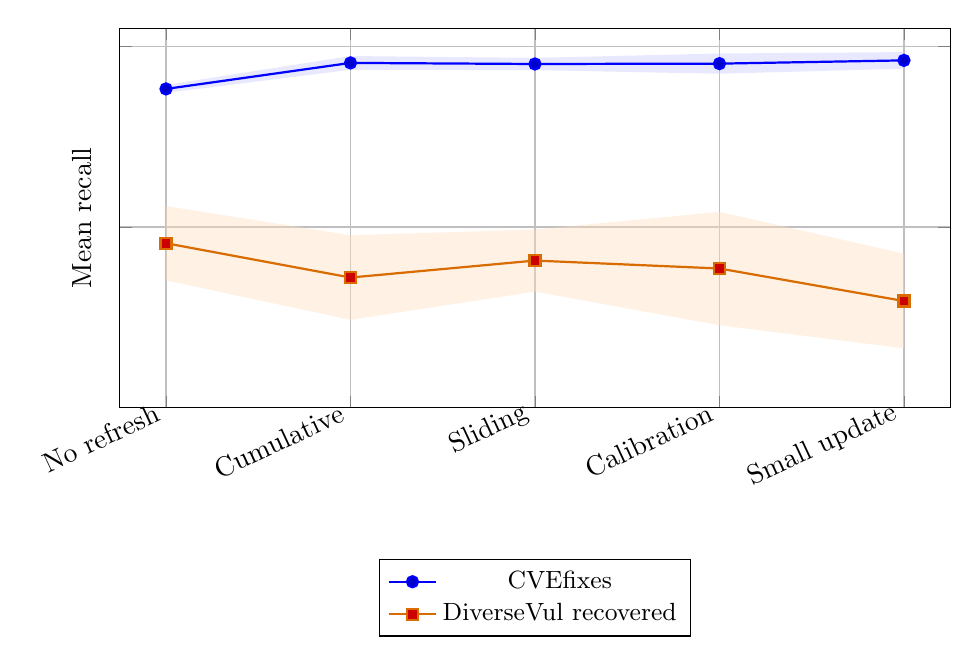
\begin{tikzpicture}
    \begin{axis}[
      width=\columnwidth,
      height=6.4cm,
      xmin=0.75,
      xmax=5.25,
      ymin=0,
      ymax=1.05,
      ylabel={Mean recall},
      yticklabel=\empty,
      xtick={1,2,3,4,5},
      xticklabels={No refresh,Cumulative,Sliding,Calibration,Small update},
      x tick label style={rotate=25,anchor=east},
      legend style={at={(0.5,-0.40)},anchor=north,font=\small},
      legend columns=1,
      grid=major
    ]
      \addplot[name path=cvemaintupper,draw=none,forget plot] coordinates {
        (1,0.893) (2,0.973) (3,0.968) (4,0.980) (5,0.984)
      };
      \addplot[name path=cvemaintlower,draw=none,forget plot] coordinates {
        (1,0.871) (2,0.935) (3,0.934) (4,0.924) (5,0.938)
      };
      \addplot[blue!20,opacity=0.45,forget plot] fill between[of=cvemaintupper and cvemaintlower];
      \addplot+[blue,thick,mark=*] coordinates {
        (1,0.882) (2,0.954) (3,0.951) (4,0.952) (5,0.961)
      };
      \addlegendentry{CVEfixes}
      \addplot[name path=dvmaintupper,draw=none,forget plot] coordinates {
        (1,0.558) (2,0.477) (3,0.493) (4,0.542) (5,0.426)
      };
      \addplot[name path=dvmaintlower,draw=none,forget plot] coordinates {
        (1,0.352) (2,0.243) (3,0.321) (4,0.228) (5,0.164)
      };
      \addplot[orange!25,opacity=0.42,forget plot] fill between[of=dvmaintupper and dvmaintlower];
      \addplot+[orange!85!black,thick,mark=square*] coordinates {
        (1,0.455) (2,0.360) (3,0.407) (4,0.385) (5,0.295)
      };
      \addlegendentry{DiverseVul recovered}
    \end{axis}
  \end{tikzpicture}
  \caption{Maintenance-policy mean recall with bootstrap uncertainty.}
  \label{fig:maintenance}
\end{figure}

\subsection{RQ4: Exploratory Monitoring Calibration}

\rqsummary{The available yearly windows do not support a mature trigger-learning
claim. CVEfixes has no violations under the chosen service event, and
recovered-date DiverseVul yields only a small 3-of-4 event pattern, so drift
alarms should be interpreted only with a pre-declared service level and action.}

Monitoring triggers are evaluated against a pre-specified recall-floor or
recall-drop event. In the CVEfixes primary run, no yearly window violates the
chosen event definition for the character baseline, so trigger precision and
recall are structurally uninformative under that service level. In the
recovered-date DiverseVul run, CWE divergence, project turnover, and unseen-token
rate each achieve precision 1.000 and recall 0.750 for the event definition,
but this corresponds to only three detected event windows out of four. RQ4 is
therefore demoted to an exploratory monitoring-calibration check. It does not
support a mature trigger-learning claim; that would require rolling-origin
replicates or another dataset to raise the number of service-level events from
single digits to dozens. The limited result is still useful as a protocol
guardrail: drift alarms should be interpreted only after an operational service
level and maintenance action have been specified.

\section{Discussion}

\subsection{What the Results Say}

The strongest result is not that every detector inevitably ages. The strongest
result is that vulnerability-detector maintenance policies and operating
points materially affect future temporal behavior under project and
label-distribution shift. The same problem can look stable, degraded, or
unusable depending on temporal cutoff, feature family, threshold policy,
project holdout, and whether independently clean negatives are included. These
are exactly the kinds of choices software maintenance research is designed to
make explicit.

\subsection{Practical Implications}

Teams deploying learning-based vulnerability detectors should:

\begin{itemize}
  \item evaluate on chronological splits and, when possible, unseen projects;
  \item report false-positive operating points rather than only maximum F1;
  \item keep independent clean functions for specificity testing;
  \item track drift in project mix, CWE mix, vocabulary, code length, and class
  prior;
  \item compare calibration, retraining, and small recent updates as explicit
  maintenance policies;
  \item define service-level triggers before interpreting drift alarms.
\end{itemize}

Table~\ref{tab:recommendations} translates these implications into concrete
maintenance choices.

\begin{table*}
\centering
\caption{Practical maintenance-policy recommendations.}
\label{tab:recommendations}
\resizebox{\textwidth}{!}{%
\begin{tabular}{p{0.22\textwidth}p{0.28\textwidth}p{0.40\textwidth}}
\toprule
Deployment condition & Recommended action & Rationale \\
\midrule
Recall is the primary service objective & Compare small recent update and
calibration-only policies. & These policies improve CVEfixes recall, but must
still be checked against false-positive cost. \\
False positives are constrained & Select thresholds with validation FPR caps
and report operating-point curves. & Best-F1 thresholds can hide high alert
rates; FPR-controlled thresholds expose the deployment tradeoff. \\
Future projects differ from training projects & Use project-held-out
validation and testing. & Ordinary chronological splits do not measure
generalization to unseen projects. \\
Training negatives are fixed code versions & Require independent clean
functions and report specificity by source. & Fixed-code negatives do not
establish arbitrary vulnerable-versus-clean behavior. \\
Drift monitors trigger an alarm & Link the alarm to a pre-declared service
event and maintenance action. & Drift alone is not failure; it becomes useful
only when tied to recall, FPR, or label-cost objectives. \\
\bottomrule
\end{tabular}
}
\end{table*}

Table~\ref{tab:alert-cost} gives the same point in operational units. It is not
a universal cost model; it simply converts FPR into expected false alerts for a
chosen review surface. Teams should replace the example surfaces with their own
pull-request or CI volumes before selecting a service-level objective.

\begin{table*}
\centering
\caption{Illustrative alert-cost conversion.}
\label{tab:alert-cost}
\small
\setlength{\tabcolsep}{4pt}
\begin{tabular}{p{0.38\linewidth}rrp{0.28\linewidth}}
\toprule
Operating condition & Clean funcs & FPR & Expected false alerts \\
\midrule
Strict validation cap & 20 per PR & 0.200 & 4.0; high but triageable \\
Cross-dataset stress & 20 per PR & 0.700 & 14.0; likely too noisy \\
CVEfixes project-held-out small update & 20 per PR & 0.945 & 18.9; nearly every clean function flagged \\
Repository-clean char4 check & 1,000 in CI & 0.845 & 845; clean benchmark failure \\
\bottomrule
\end{tabular}
\end{table*}

\section{Threats to Validity}

\textbf{Construct validity of labels.} CVEfixes compares vulnerable and fixed
versions of changed code. This is a meaningful pre/post-fix task, but it is not
the same as arbitrary vulnerable-versus-clean detection. Claims based on
CVEfixes must therefore be read as claims about pre/post-fix detection unless
they are supported by independent clean examples. The independent-clean
challenge shows that CVEfixes-trained models can retain high temporal recall
while having poor external clean specificity.

\textbf{Temporal metadata.} CVEfixes has explicit temporal metadata in the local
mirror. DiverseVul requires enrichment from external repository metadata. The
recovery pass substantially improves coverage, but 10,478 local rows still lack
recovered dates (Table~\ref{tab:diversevul-accounting}). We therefore use
recovered-date DiverseVul as sensitivity evidence and exclude unrecovered rows
from temporal claims rather than mixing proxy and recovered dates. This choice
sacrifices coverage to avoid a more damaging validity problem: treating
heterogeneous date sources as if they were equivalent.

\textbf{Commit-date external replication.} PrimeVul-paired adds a third
dataset with recovered commit dates rather than CVE-year proxy dates. Coverage
is partial: 494 commit pages are recovered, yielding 1,267 post-deduplication
rows from 74 projects. Its results are therefore used as external sensitivity
evidence, not as a replacement primary dataset. The paired construction also
means the task remains pre/post-fix detection, not arbitrary
vulnerable-versus-clean detection.

\textbf{Detector-family validity.} The study includes lightweight baselines,
frozen CodeBERT, calibrated LineVul, and full-dataset fine-tuning. Bounded
fine-tuning is retained only as an artifact-level execution check because its
sample size, one-epoch schedule, and maximum length 128 are too limited for
architecture comparison. The recovered-date DiverseVul neural collapse is
primarily a threshold-policy artifact: the fixed-FPR validation rule selects a
near-all-negative threshold even though the ranking metrics are non-random.
The PrimeVul-paired recovered-date neural rerun addresses part of this concern
by retaining training curves, validation losses, validation AUPRC/AUROC, and
validation threshold curves under five requested epochs, length-256,
class-balanced fine-tuning on all eligible recovered-date rows. It remains
diagnostic, however, not a definitive neural architecture comparison. A
stronger neural operating-point claim would require a larger learning-rate
sweep, external prospective validation, and additional detector families such
as CodeT5, UniXcoder, graph-based vulnerability detectors, and multi-modal
vulnerability models. The contribution is therefore a maintenance-evaluation
framework and empirical stress test, not a claim that the evaluated neural
architectures exhaust the state of the art.

\textbf{Leakage controls.} Exact duplicates are removed before splitting, and
near-duplicate-controlled reruns remove future records close to earlier
windows. Approximate matching thresholds may still under-match semantic clones
or over-match short boilerplate functions.

\textbf{Project and group validity.} The grouped audit finds no train-to-future
commit-group or vulnerable/fixed-pair overlap in controlled runs, and the
full-dataset neural rerun reports unseen-project temporal evaluation. The
classical maintenance-policy rerun applies the same unseen-project temporal
constraint, although its logistic models are bounded and sampled for tractable
reruns. These project-held-out classical policies reveal very high FPR on
CVEfixes, so their recall gains should be interpreted as maintenance tradeoffs,
not improvements at an acceptable operating point by themselves.

\textbf{Statistical validity.} Annual temporal windows are few, so correlations
between drift and recall should be read as descriptive associations. We report
the number of windows, confidence intervals for correlations, permutation tests,
and Holm-adjusted values over the drift-signal family, but these tests still do
not establish causality.

\section{Conclusion}

This article introduced MAINT-VD, a maintenance-evaluation framework for
studying learning-based vulnerability detectors as maintained software
artifacts. A deployed detector has a lifecycle: it is
trained on historical projects, calibrated on a validation set, operated at a
chosen threshold, monitored against future code, and periodically refreshed or
revalidated as the surrounding software ecosystem changes. Treating these
decisions as part of the detector turns temporal evaluation into a software
maintenance problem.

The empirical results support a precise conclusion: maintenance policies and
threshold rules are part of detector behavior under project and
label-distribution shift; temporal recall is meaningful only when reported with
false-positive and clean-specificity evidence. The evidence is not a simple
story that every detector ages monotonically. On
CVEfixes, the primary character baseline remains relatively stable in ordinary
temporal evaluation, and low-cost recent updates improve already strong recall.
Under project-held-out temporal testing, however, classical refresh policies
obtain high recall at very high false-positive rates. Full-dataset CodeBERT and
LineVul runs show the same lesson from a neural perspective: AUROC and AUPRC
summarize ranking behavior, but maintenance decisions require precision, recall,
F1, specificity, and FPR at explicit operating points.
PrimeVul-paired strengthens the external-validity story without changing this
conclusion: after commit-date recovery, it provides a smaller but true-dated
paired sensitivity study. Classical models still trade recall against high FPR,
and the fuller neural rerun shows that retained training curves and more
complete local training do not by themselves create a reliable future-project
operating point.

The study also exposes two validity lessons for future vulnerability-detector
research. First, fixed-code negatives are not sufficient evidence of clean-code
specificity. The independent-clean challenge shows that a model can preserve
future recall on a pre/post-fix task while flagging many independently clean
functions. Second, temporal evidence depends on metadata quality. CVEfixes can
serve as the primary temporal study because explicit dates are available in the
local mirror. DiverseVul becomes much more useful after repository-date
recovery, but remaining missingness still makes it better suited to sensitivity
evidence than to the article's primary claim. These points sharpen rather than
weaken the maintenance thesis: they specify the empirical conditions under
which the thesis can be defended.

For practitioners, the implication is operational. A vulnerability detector
should be deployed with a declared service level, a threshold-selection rule,
an independent clean evaluation set, drift monitors, and a planned policy for
calibration or retraining. For researchers, the implication is methodological:
MAINT-VD is a reusable evaluation scaffold, not a final ranking of detector
architectures. Temporal splits, project-held-out evaluation, near-duplicate
controls, operating-point curves, and label-cost reporting should accompany
claims about security-detector robustness. A single random split or a single
F1-optimized threshold is not enough to describe how a detector will behave as
software projects evolve.

Future work should recover repository commit dates for additional datasets,
including Big-Vul and language-specific corpora such as Vul4J~\cite{bui2022vul4j},
extend the clean-function challenge across more languages and project sources,
evaluate larger neural tuning budgets, and test the monitoring triggers in
prospective or continuously updated settings. The broader goal is to make
learning-based security tools auditable over time. Security detectors will be
most useful when their maintenance assumptions are visible, measurable, and
revisable like the assumptions of other software engineering infrastructure.

\printcredits

\section*{Declaration of Competing Interest}

The authors declare no known competing financial interests or personal
relationships that could have appeared to influence the work reported in this
article.

\section*{Code Availability}

The source code, experiment scripts, manuscript sources, and replication
materials are available in the GitHub repository
\href{https://github.com/LeoTTTPhat/MAINT-VD}
{\texttt{https://github.com/LeoTTTPhat/MAINT-VD}}.
The repository should be archived with a DOI or immutable release tag before
final submission so that the released artifact version matches the checksums
reported in the repository manifest.

\section*{Acknowledgement}

We acknowledge the support of time and facilities from Ho Chi Minh City
University of Technology (HCMUT), VNU-HCM for this study.

\bibliographystyle{elsarticle-num}
\bibliography{references}

\end{document}
